\documentclass[8pt,landscape, a4paper]{extarticle}
\usepackage{multicol}
\usepackage{calc}
\usepackage{xspace}
\usepackage{ifthen}
\usepackage[landscape]{geometry}
\usepackage[dvipsnames]{xcolor}
\usepackage{hyperref}
\usepackage{tikz}
\usepackage{polynom}
\usepackage{pifont}
\usepackage{amssymb}
\usepackage{setspace}
\usepackage{dsfont}

% my packages:
\usepackage{amsmath, amssymb, amsfonts, amsthm, mathtools}
\usepackage{tcolorbox}
\usepackage[utf8]{inputenc}
\usepackage{enumitem}
\usepackage{physics}
\usepackage{wrapfig}
%framed boxes
\usepackage{mdframed}
\usepackage{array}
\usepackage{tcolorbox}
\usepackage{accents}

%for images
\usepackage{graphicx}

% This sets page margins to .6cm
\geometry{top=-0.1cm,left=0.cm,right=0.cm,bottom=0.1cm}

% Turn off header and footer
\pagestyle{plain}
% Turn off page numbering
\pagenumbering{gobble}

% Redefine section commands to use less space
\makeatletter
\renewcommand{\section}{\@startsection{section}{1}{0mm}%
                                {-1ex plus -.5ex minus -.2ex}%
                                {0.5ex plus .2ex}%x
                                {\normalfont\large\bfseries}}
\renewcommand{\subsection}{\@startsection{subsection}{2}{0mm}%
                                {-1ex plus -.5ex minus -.2ex}%
                                {1ex plus .2ex}%
                                {\normalfont\small\bfseries}}
\renewcommand{\subsubsection}{\@startsection{subsubsection}{3}{0mm}%
                                {-1ex plus -.5ex minus -.2ex}%
                                {1ex plus .2ex}%
                                {\normalfont\small\bfseries}}
\makeatother

% Don't print section numbers
\setcounter{secnumdepth}{1}

\setlength{\parindent}{0pt}
\setlength{\parskip}{0pt plus 0.5ex}
% define box
\tikzstyle{fancytitle} =[fill=black, text=white, font=\footnotesize\bfseries]

\usepackage{color}
\definecolor{light}{rgb}{0.5, 0.5, 0.5}
\def\light#1{{\color{light}#1}}

% -----------------------------------------------------------------------

\begin{document}
\raggedright
\footnotesize
\begin{multicols*}{3}

% multicol parameters
% These lengths are set only within the two main columns
\setlength{\columnseprule}{0.25pt}
\setlength{\premulticols}{1pt}
\setlength{\postmulticols}{1pt}
\setlength{\multicolsep}{1pt}
\setlength{\columnsep}{2pt}


% main heading
\begin{center}
	\Large{\textbf{Optimization for Data Science}} \\
    \small{by Nils Jensen in FS23 - No guarantee of completeness}
\end{center}


\newcommand\R{\mathbb{R}}
\newcommand\E{\mathbb{E}}
\newcommand\Q{\mathbb{Q}}
\newcommand\N{\mathbb{N}}
\newcommand\C{\mathbb{C}}
\newcommand\X{\mathcal{X}}
\newcommand\Y{\mathcal{Y}}
\newcommand\D{\mathcal{D}}
\newcommand{\veca}{\mathbf{a}}
\newcommand{\bb}{\mathbf{b}}
\newcommand{\vecd}{\mathbf{d}}
\newcommand{\ee}{\mathbf{e}}
\newcommand{\vecg}{\mathbf{g}}
\newcommand{\mm}{\mathbf{m}}
\newcommand{\vecs}{\mathbf{s}}
\newcommand{\uu}{\mathbf{u}}
\newcommand{\vv}{\mathbf{v}}
\newcommand{\ww}{\mathbf{w}}
\newcommand{\xx}{\mathbf{x}}
\newcommand{\yy}{\mathbf{y}}
\newcommand{\zz}{\mathbf{z}}
\newcommand{\rr}{\mathbf{r}}
\newcommand{\ssigma}{\boldsymbol{\sigma}}
\newcommand{\xxi}{\boldsymbol{\xi}}
\newcommand{\eeta}{\boldsymbol{\eta}}
\newcommand\Max{\mathrm{Max}}
\newcommand\argmin{\mathrm{argmin}}
\newcommand\relint{\mathrm{relint}}
\newcommand\argmax{\mathrm{argmax}}
\newcommand\prox{\mathrm{prox}}
\newcommand\Var{\mathrm{Var}}
\newcommand\Cov{\mathrm{Cov}}
\newcommand\conv{\mathrm{conv}}
\newcommand\diam{\mathrm{diam}}
\newcommand\sgn{\mathrm{sgn}}
\newcommand{\dom}{\textbf{dom}}
\newcommand\Min{\mathrm{Min}}
\newcommand\Limit{\lim_{n \rightarrow \infty}}
\newcommand\Sup{\mathrm{Sup}}
\newcommand\lmo{\mathrm{LMO}}
\newcommand\Inf{\mathrm{Inf}}
\newcommand\Def{\textbf{Def.}\hspace{3mm}}
\newcommand\Bsp{\textit{Bsp.}\hspace{2mm}}
\newcommand\Satz{\textbf{{Satz.}}\hspace{3mm}}
\newcommand\Kor{\textbf{Kor.}\hspace{3mm}}
\newcommand\Bem{\textbf{Bem.}\hspace{3mm}}
\newcommand\converges[2]{\underset{#1\rightarrow #2}{\longrightarrow}}
\newcommand{\BigO}{\mathcal{O}}

\newcommand\Sum{\sum\limits}
\newcommand\Lim{\lim\limits}
\newcommand\Int{\int\limits}

\newcommand\Reihe{\sum_{k = 1}^{\infty}}

\newcommand\Ib{\overline{I}}

\newcommand*\diff{\mathop{}\!\mathrm{d}}

\newcommand\Title[1]{\vspace{.1mm}\begin{tikzpicture} \node[fancytitle, right=10pt, fill=gray] {#1}; \end{tikzpicture}}

\everymath{\color{PineGreen}}

\newcommand{\ubar}[1]{\underaccent{\bar}{#1}}

%\renewcommand{\(}{\relax\ifmmode\@badmath\else\color{blue}$\fi}
%\renewcommand{\)}{\relax\ifmmode\ifinner$\color{black}\else\@badmath\fi\else \@badmath\fi }
%\catcode`\$=13
%\def${\ifmmode)\xspace\else(\fi} 
%\makeatother

\scriptsize

\newenvironment{framed}
{\begin{tcolorbox}[colback=orange!10!white,
                   colframe=black, 
                   boxrule=0.5pt,
                   enlarge top by=0cm, 
                   enlarge bottom by=0cm, 
                   boxsep=-2mm]}
		{\end{tcolorbox}}

% _____ BEGINNING OF DOCUMENT __________________________________________________

\section{Introduction}
\Title{Expected risk minimization}
We have a \textbf{data source} $\mathcal{X}$ from which we draw \textbf{samples} $X_1, \dots, X_n$. We can see $\mathcal{X}$ as a probability distribution. Define $\mathcal{H}$ as a class of \textbf{hypotheses} (possible explanations of $\mathcal{X}$). Want to select the one that best explains $\mathcal{X}$. \\
A \textbf{risk/loss function} $l : \mathcal{H} \times \mathcal{X} \rightarrow \R$ quantifies how well we think that a given hypothesis $H \in \mathcal{H}$ explains given data $X \in \mathcal{X}$. \\
The \textbf{expected risk} is $l(H) := \E_{\mathcal{X}}[l(H, X)]$. Goal: Find $H \in \mathcal{H}$ with the smallest expected risk: $H^* = \argmin_{H \in \mathcal{H}} l(H)$.
Problem: We do not know the distribution: we can only work with finitely many samples. We try to be \textbf{probably approximately correct (PAC)}: take tolerances $\delta, \epsilon > 0$, we want to produce a hypothesis $\Tilde{H} \in \mathcal{H}$ such that $l(\Tilde{H}) \leq \inf_{H \in \mathcal{H}}{l(H)} + \epsilon$.\\
\Title{Empirical risk minimization}
We have \textbf{training data} $X_1, \dots, X_n$ from which we compute the \textbf{empirical risk}: $l_n(H) = \frac{1}{n}\sum_{i=1}^n{l(H, X_i)}$ of a hypothesis $H$. For $n \rightarrow \infty$, this converges to $l(H)$. Formally the \textbf{weak law of large numbers} states, that for $H \in \mathcal{H}$ and $\delta, \epsilon > 0$ we have $n_0$ such that for $n_0 \geq n$ we have $\abs{l_n(H) - l(H)} \leq \epsilon$ with probability at least $1 - \delta$. \\
We use \textbf{empirical risk minimization} as a proxy for risk minimization: For $n \in \N$ and $X_1, \dots, X_n \sim \X$ produce a hypothesis $\Tilde{H}_n$ such that $l_n(\Tilde{H}_n) \leq \inf_{H \in \mathcal{H}}{l_n(H)} + \epsilon$. \\
\textbf{Careful:} Empirical risk does \textit{not} always converge to expected risk(!).
\Title{The map of learning}
\begin{wrapfigure}[18]{l}{0.12\textwidth}
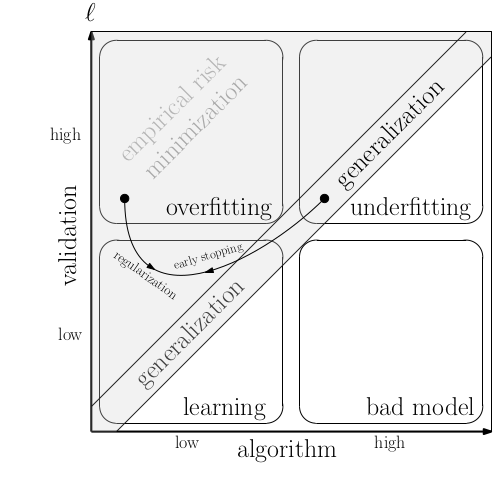
\includegraphics[scale=0.2]{ODS/images/map_of_learning.png}
\end{wrapfigure}
\textbf{Algorithm}: computational procedure according to which a hypothesis $H_n$ is obtained from training data $X_1, \dots, X_n$. \\
\textbf{Validation}: Once a hypothesis $H_n$ has been obtained through training, one also needs to assess its expected risk, i.e. locate $H_n$ in the $l$-dimension. Using the weak law of large numbers, $l(H_n)$ can be estimated via its empirical risk on test data—fresh samples from $\mathcal{X}$ that the algorithm has not seen. \\
\textbf{Overfitting}: If our learning algorithm returns a hypothesis with low empirical risk but high expected risk, we have a case of overfitting. The main cause of overfitting is that our theory (hypothesis class $\mathcal{H}$ and loss function $l$) is so complex that it allows us to almost perfectly explain any training data. \\
\textbf{Underfitting}: If the learning algorithm returns a hypothesis with high empirical risk, we cannot even explain the training data. In this case, there is no justified hope to be able to explain unseen data. The main cause of underfittting is that our theory is too simple to capture the nature of the data. \\
\textbf{Learning}: If both empirical and expected risk are low, we can make a case that we have learned something. \\
\textbf{Generalization}: Ideally, the expected risk is close to the empirical risk, and if this happens, we have generalization. This means that the hypothesis explains unseen data equally well as the training data. But it does \textit{not} mean that the explanation is good. \\
\textbf{Regularization}: In the case that overfitting is observed, a possible remedy is to add a regularization term $r$ to the loss function $l$ with the goal of \textit{punishing} complex hypotheses. Empirically minimizing $l' = l + \lambda r$ for a real number $\lambda > 0$ therefore has the effect that we introduce a \textbf{bias}, meaning that we deviate more and more from our theory, with the effect that the empirical risk increases. But as the intended consequence, the \textbf{variance} (sensitivity to the training data) decreases, and this may reduce the expected risk. \\
\Title{Worst-case versus average-case complexity} 
The classical measure of algorithm performance is its \textbf{worst-case complexity}, the function that maps $n$ to the maximum runtime of the algorithm over all possible inputs of size $n$. The \textbf{average case complexity} is the function that maps $n$ to the expected runtime of the algorithm, taken over its input distribution. \\
\Title{The estimation-optimization tradeoff} 
As we inevitably lose precision in going from empirical to expected risk, it doesn’t help to optimize the empirical risk to a significantly higher precision. Let us call the precision that we lose in going from empirical to expected risk the \textbf{estimation error}; the precision we lose in finding only an almost best explanation of the training data is the \textbf{optimization error}. In small-scale learning, it doesn’t hurt to go for as small an optimization error as we can. But in large-scale learning, we may need to give up on some optimization precision in order to be able to stay within the optimization time budget. The \textbf{estimation-optimization tradeoff} consists in finding the most efficient way of spending the resources under the given constraints.
\section{Theory of Convex Functions}
\Title{Mathematical Background} 
\textbf{Cauchy-Schwarz Inequality}: $\abs{\uu^T \vv} \leq \norm{\uu} \norm{\vv}$. We have equality if and only if $\uu$ and $\vv$ are colinear. \\
\textbf{Cosine Theorem}: $2\vv^T \ww = \norm{\vv}^2 + \norm{\ww}^2 - \norm{\vv - \ww}^2$ \\
The \textbf{spectral norm} of a matrix $A$ is: $\norm{A} := \max_{\vv \in \R^d, \vv \neq 0}{\frac{\norm{A\vv}_2}{\vv}_2} = \max_{\norm{\vv}_2=1}{\norm{A\vv}_2}$. \\
It follows that $\norm{A \vv}_2 \leq \norm{A} \norm{\vv}_2$ for all $\vv$. \\
\textbf{Mean value theorem}: Let $a < b$ and $h: [a, b] \rightarrow \R$ be a continuous function which is differentiable on $(a, b)$. Then there exists a $c \in (a, b)$ such that: $h'(c) = \frac{h(b) - h(a)}{b - a}$. \\
Let $f : \dom(f) \rightarrow \R^m$ where $\dom(f) \subset \R^d$. The function $f$ is called \textbf{differentiable} at $\xx$ if there exists a $(m \times d)$-matrix $A$ and an error function $r : \R^d \rightarrow \R^m$ defined in some neighborhood of $\mathbf{0} \in \R^d$ such that for all $\yy$ in a neighborhood of $\xx$: $f(\yy) = f(\xx) + A(\yy - \xx) + r(\yy - \xx)$ where $\lim_{\vv \rightarrow 0}{\frac{\norm{r(\vv)}}{\norm{v}}} = 0$. $A$ is unique and called the \textbf{jacobian} of $f$ at $\xx$. We denote it $Df(x)$ and have $D f(\xx)_{i, j} = \frac{\partial f_i}{\partial x_j}(\xx)$.\\
For $m=1$ (i.e $f : \R^d \rightarrow \R)$ we call the jacobian the \textbf{gradient} of $f$ and denote it $\nabla f^T$. Geometrically, this means that the graph of the affine function $f(x) + \nabla f(\xx)^T$ is a tangent hyperplane to the graph of $f$ at $(\xx, f (\xx))$. \\
\textbf{Chain Rule}: $D(f \circ g)(\xx) = D f(g(\xx)) Dg(\xx)$. \\
\Title{Convex Sets} 
A set $C \subset \R^d$ is \textbf{convex} if for any two points $\xx, \yy \in C$ the connecting line segment is in $C$. In formula this means for all $\lambda \in [0, 1]$: $\lambda \xx + (1 - \lambda) \yy \in C$. \\
\textbf{Intersection of convex sets}: Let $C_i$, $i \in I$ be convex sets, where $I$ is a (possibly infinite) index set. Then $C = \cap_{i \in I}{C_i}$ is a convex set. 
\begin{framed}
    \textbf{Mean value inequality}: Let $f : \dom(f) \rightarrow \R^m$ be differentiable, $X \subset \dom(f)$ a convex, nonempty and open set, $B > 0$. The following are equivalent:
    \begin{enumerate}[label=(\roman*), topsep=0pt,itemsep=0ex,partopsep=0ex,parsep=0ex]   
        \itemsep0em
        \item $f$ is $B$-Lipschitz: $\forall \xx, \yy \in X : \norm{f(\xx) - f(\yy)} \leq B \norm{\xx - \yy}$
        \item $f$ has differentials bounded by $B$ (in spectral norm): $\forall \xx \in X: \norm{D f(\xx)} \leq B$.
    \end{enumerate}
    (ii) $\implies$ (i) even if $X$ is not open.
\end{framed}
\Title{Convex functions} 
\begin{framed}
    A function $f$ as above is said to be \textbf{convex} if $\dom(f)$ is convex and for all $\xx, \yy \in \dom(f)$ and $\lambda \in [0, 1]$ we have: $f(\lambda \xx + (1 - \lambda)\yy) \leq \lambda f(\xx) + (1 - \lambda) f(\yy)$.   
\end{framed}
While the graph of $f$ is the set $\{(\xx, f (\xx)) \in \R^{d+1} : \xx \in \dom(f)\}$, the \textbf{epigraph} is the set of points above the graph, $\textbf{epi}(f) := \{(\xx, \alpha) \in \R^{d+1} : \xx \in \dom(f), \alpha \geq f(\xx)\}$. $f$ is a convex function if and only if $\textbf{epi}(f)$ is a convex set. \\
\textbf{Jensen's inequality} Let $f : \R^d \rightarrow \R$ be a convex function, $\xx_1, \dots, \xx_n \in \dom(f)$ and $\lambda_1, \dots, \lambda_m \in \R_{+}$ such that $\sum_{i=1}^n{\lambda_i}=1$, then: $f\left(\sum_{i=1}^m{\lambda_i x\xx_i} \right) \leq \sum_{i=1}^n{\lambda_i f(\xx_i)}$. \\
If $f$ is convex and $\dom(f)$ is open then $f$ is continuous.\\
\begin{framed}
    \textbf{First-order characterization of convexity} Let $\dom(f)$ be open and $f$ differentiable then $f$ is convex if and only if $\dom(f)$ is convex and $f(\yy) \geq f(\xx) + \nabla f(\xx)^T (\yy - \xx)$. Geometrically, this means that for all $\xx \in \dom(f)$, the graph of $f$ lies above its tangent hyperplane at the point $(\xx, f(\xx))$.
\end{framed}
\textbf{Monotonicity of the gradient}: Suppose that $\dom(f)$ is open and that $f$ is differentiable. Then $f$ is convex if and only if $\dom(f)$ is convex and $(\nabla f(\yy) - \nabla f(\xx))^T (\yy - \xx) \geq 0$ holds for all $\xx, \yy \in \dom(f)$.
\begin{framed}
    \textbf{Second-order characterization of convexity} Suppose that $\dom(f)$ is open and that $f$ is twice differentiable; in particular, the Hessian (matrix of second partial derivatives) exists at every point $\xx \in \dom(f)$ and is symmetric. Then $f$ is convex if and only if $\dom(f)$ is convex, and for all $\xx \in \dom(f)$, we have $\nabla^2 f(\xx) \succcurlyeq 0$ (psd).
\end{framed}
\textbf{Operations that preserve convexity}: Let $f_1, \dots, f_n$ be convex functions and $\lambda_1, \dots, \lambda_n \in \R_{+}$. Then $f := \max_{i=1}^m{f_i}$ and $f := \sum_{i=1}^n{\lambda_i f_i}$ are convex on $\dom(f) = \cap_{i=1}^n{\dom(f_i)}$. Furthermore let $f$ be convex with $\dom(f) \subset \R^d$ and $g : \R^m \rightarrow \R^d$ be an affine function (i.e. $g(\xx) = A \xx + \bb$. Then $f \circ g$ is convex on $\dom(f \circ g) = \{ \xx \in \R^m : g(\xx) \in  \dom(f)\}$.\\
\Title{Minimizing convex functions} 
A \textbf{local minimum} of $f: \dom(f) \rightarrow \R$ is a point $\xx$ such that there exists $\epsilon > 0$ with: $f(\xx) \leq f(\yy)$ for all $\yy \in \dom(f)$ with $\norm{\yy - \xx} < \epsilon$. \\
Let $x^*$ be a local minimum of a convex function $f : \dom(f) \rightarrow \R$. Then $x^*$ is a global minimum, meaning that $f (x^*) \leq f(y) \forall y \in \dom(f)$. \\
Suppose that $f : \dom(f) \rightarrow \R$ is convex and differentiable over an open domain $\dom(f) \subset \R^d$. Let $x \in \dom(f)$. If $\nabla f(\xx) = 0$, then $\xx$ is a global minimum. \\
Suppose that $f : \dom(f) \rightarrow \R$ is differentiable over an open domain $\dom(f) \subset \R^d$ . Let $\xx \in \dom(f)$. If $\xx$ is a global minimum then $\nabla f(\xx) = 0$. \\
\Title{Strictly convex functions} 
A function $f : \dom(f) \rightarrow \R$ is \textbf{strictly convex} if $\dom(f)$ is convex and for all $\xx \neq \yy \in \dom(f)$ and all $\lambda \in (0, 1)$, we have $f(\lambda \xx + (1 - \lambda)\yy) < \lambda f(\xx) + (1 - \lambda) f(\yy)$. \\
Suppose that $\dom(f)$ is open and that $f$ is twice continuously differentiable. If the Hessian $\nabla^2 f(\xx) \succ 0$ for every $\xx \in \dom(f)$, then $f$ is strictly convex. \\
Let $f : \dom(f) \rightarrow \R$ be strictly convex then $f$ has at most one global minimum. \\
\Title{Constrained Minimization} 
Let $f : \dom(f) \rightarrow \R$ be convex and $X \subset \dom(f)$ be a convex set. A point $\xx$ is a \textbf{minimizer} of $f$ over $X$ if $f(\xx) \leq f(\yy), \forall \yy \in X$. \\
Suppose that $f : \dom(f) \rightarrow \R$ is convex and differentiable over an open domain $\dom(f) \subset \R^d$, and let $X \subset \dom(f)$ be a convex set. A point $\xx^* \in X$ is a minimizer if and only if $\forall \xx \in X : \nabla f(\xx^*)^T (\xx - \xx^*) \geq 0$.
\Title{Existence of a minimizer}
Let $f : \R^d \rightarrow \R$ and $\alpha \in \R$. The set $f^{\leq \alpha} := \{\xx \in \R^d: f(\xx) \leq \alpha\}$ is the \textbf{$\alpha$-sublevel set} of $f$. \\
\textbf{Weierstrass Theorem}: Let  $f : \R^d \rightarrow \R$ be a continuous function and suppose there is a non-empty and bounded sublevel set $f^{\leq \alpha}$. Then $f$ has a global minimum. \\
\Title{Convex programming}
An \textbf{optimization problem} in standard form is given by: 
\begin{align*}
    \text{minimize }   &f_0(\xx) \\
    \text{subject to } &f_i(\xx) \leq 0, i=1, \dots m \\
                       &h_i(\xx) = 0 i=1, \dots, p
\end{align*}
A \textbf{convex program} arises when the $f_i$ are convex functions and the $h_i$ are affine functions with domain $\R^d$. We call the region $X = \{\xx \in \R^d : f_i(\xx)\leq 0, i=1, \dots, m; h_i(\xx) =0, i=1, \dots p\}$ the \textbf{feasible region}, in this case it is a convex set. \\
The \textbf{Lagrangian} is the functional $L : \mathcal{D} \times \R^m \rightarrow \R$ given by: $L(\xx, \mathbb{\lambda}, \mathbb{\nu}) = f_0(\xx) + \sum_{i=1}^m{\lambda_i f_i(\xx)} + \sum_{i=1}^p{\nu_i h_i(\xx)}$. We call the $\lambda_i, \nu_i$ are called \textbf{Lagrange multipliers}. The Lagrange \textbf{dual function} is $g : \R^m \times \R^p \rightarrow \R \cup \{- \infty\}$ defined by $g(\mathbb{\lambda}, \mathbb{\nu}) = \inf_{\xx \in D} L(\xx, \mathbb{\lambda}, \mathbb{\nu})$. \\
\textbf{Weak duality} If $\xx$ is a feasible solution then $g(\mathbb{\lambda}, \mathbb{\nu}) \leq f_0(\xx)$, for all $\mathbb{\lambda} \in \R^m, \mathbb{\nu} \in \R^p$ with $\mathbb{\lambda} \geq 0$. \\
The \textbf{Lagrangian dual problem} is given by:
\begin{align*}
    \text{maximize }   g(\mathbb{\lambda}, \mathbb{\nu}) && \text{subject to }  \mathbb{\lambda} \geq 0
\end{align*}
The equivalent minimization is always a convex program (even if the original program was not). \\
\textbf{Slaters Condition}: If there is a Slater's point $\Tilde{\xx}$ (a point which satisfies all inequality constraints of the original program strictly), then the infimum value of the primal equals the supremum value of its Lagrange dual. Moreover, if this value is finite, it is attained by a feasible solution of the dual. This is called \textbf{strong duality}. \\
\textbf{Karush-Kuhn-Tucker necessary conditions} Let $\Tilde{\xx}$ and $(\Tilde{\mathbb{\lambda}}, \Tilde{\mathbb{\nu}})$ be feasible solutions of the primal optimization problem and its Lagrangian dual repectively with zero duality gap. If all $f_i$ and $h_i$ are differentiable then: $\Tilde{\lambda}_i f_i(\Tilde{\xx}) = 0 $ for $i=1, \dots, m$ and $\nabla f_0(\Tilde{\xx}) + \sum_{i=1}^m{\Tilde{\lambda}_i \nabla f_i(\Tilde{\xx})} + \sum_{i=1}^p{\Tilde{\nu}_i \nabla h_i(\Tilde{\xx})} = 0$. \\
\textbf{Karush-Kuhn-Tucker sufficient conditions} The KKT necessary conditions are sufficient to ensure strong duality if all $f_i, h_i$ are differentiable and the $f_i$ are convex and the $h_i$ affine.

\section{Gradient Descent}
\Title{Overview}
Number of steps is given which the respective variant needs on the respective function class to achieve additive approximation error at most $\epsilon$.
\newcolumntype{P}[1]{>{\centering\arraybackslash}p{#1}}
\begin{center}
    \begin{tabular}{ |P{10em}|P{5em}|P{5em}|P{5em}|P{5em}| } 
     \hline
        & Lipschitz convex functions & smooth convex functions & strongly convex functions & smooth and strongly convex functions \\ 
        \hline
        gradient descent & $\BigO(1/\epsilon^2)$ & $\BigO(1/\epsilon)$ & & $\BigO(\log \left(1/\epsilon\right))$ \\
        \hline
        accelerated gradient descent & & $\BigO(1 / \sqrt{\epsilon})$ & & \\
        \hline
        projected gradient descent & $\BigO(1 / \epsilon^2)$ & $\BigO(1 / \epsilon)$ & & $\BigO(\log(1 / \epsilon)$ \\
        \hline
        subgradient descent & $\BigO(1 / \epsilon^2)$ & & $\BigO(1 / \epsilon)$ & \\
        \hline
        stochastic gradient descent & $\BigO(1 / \epsilon^2)$ & & $\BigO(1 / \epsilon)$ & \\
        \hline
    \end{tabular}
\end{center}
\Title{Vanilla Gradient Descent}
\begin{framed}
    Each step of \textbf{gradient descent} is defined as: $\xx_{t+1} = \xx_t - \gamma \nabla f(\xx_t)$. Where $\gamma$ is a fixed \textbf{stepsize}.
\end{framed}
The \textbf{vanilla analysis} of gradient descent yields with $\vecg_t = \nabla f(\xx_t)$: $\sum_{t=0}^{T-1}{(f(\xx_t) - f(\xx^*))} \leq \frac{\gamma}{2}\sum_{t=0}^{T-1}{\norm{\vecg_t}^2} + \frac{1}{2 \gamma}\norm{\xx_0 - \xx^*}^2$. Trick: use cosine theorem and first order characterisation of convexity. \\
\Title{Lipschitz convex functions}
\textbf{Theorem}: Let $f : \R^d \rightarrow \R$ be convex and differentiable with a global minimum $\xx^*$. Suppose that $\norm{\xx_0 - \xx^*} \leq R$ and $\norm{\nabla f(\xx)} \leq B$ for all $\xx$. With stepsize $\gamma = \frac{R}{B\sqrt{T}}$ we get: $\frac{1}{T}\sum_{t=0}^{T-1}{(f(\xx_t) - f(\xx^*))} \leq \frac{RB}{\sqrt{T}}$. \\
\Title{Smooth convex functions}
\begin{framed}
    Let $f : \dom(f) \rightarrow \R$ be a differentiable function and $X \subset \dom(f)$ be convex and $L \in \R_{+}$. $f$ is called \textbf{smooth} over $X$ if: 
    \begin{align*}
         f(\yy) \leq f(\xx) + \nabla f(\xx)^T (\yy - \xx) + \frac{L}{2}\norm{\xx - \yy}^2 && \forall \xx, \yy \in X
    \end{align*}
\end{framed}
\textbf{Alternative characterisation of smoothness}: Suppose that $\dom(f)$ is open and convex and that $f$ is differentiable then the following are equivalent:
\begin{enumerate}[label=(\roman*), topsep=0pt,itemsep=0ex,partopsep=0ex,parsep=0ex]
    \itemsep0em
    \item $f$ is smooth with parameter $L$.
    \item $g(\xx) = \frac{L}{2} \xx^T \xx - f(\xx)$ is convex over $\dom(g) = \dom(f)$.
\end{enumerate}
Suppose that $f : \R^d \rightarrow \R$ is convex and differentiable, then the following two statements are equivalent:
\begin{enumerate}[label=(\roman*), topsep=0pt,itemsep=0ex,partopsep=0ex,parsep=0ex]    
    \itemsep0em
    \item $f$ is smooth with parameter $L$.
    \item $\norm{\nabla f(\xx) - \nabla f(\yy)} \leq L \norm{\xx -\yy}$ for all $\xx, \yy \in \R^d$.
\end{enumerate}
\textbf{Operations that preserve convexity} Let $f_1, \dots, f_n$ be smooth with parameters $L_1, \dots, L_n$ and let $\lambda_1, \dots, \lambda_n \in \R_{+}$. Then $f := \sum_{i=1}^n{\lambda_i f_i}$ is smooth with parameter $\sum_{i=1}^n{\lambda_i L_i}$. Furthermore if $f : \dom(f) \rightarrow \R$ is smooth with parameter $L$ and $g : \R^m \rightarrow \R^d$ is an affine function $g(\xx) = A\xx +\bb$, then $f \circ g$ is smooth with parameter $L \norm{A}^2$. \\
\textbf{Sufficient decrease} Let $f : \R^d \rightarrow \R$ be differentiable and smooth with parameter $L$, and $\gamma = \frac{1}{L}$, then gradient descent satisfies: $f(\xx_{t+1}) \leq f(\xx_t) - \frac{1}{2L}\norm{\nabla f(\xx_t)}^2$. \\
\textbf{Theorem}: The above yields $f(\xx_T) - f(\xx^*) \leq \frac{L}{2T}\norm{\xx_0 - \xx^*}^2$. Trick use vanilla analysis to bound the sum of $g_t$. \\
\Title{Accelerated Gradient Descent}
\begin{framed}
    Choose $\zz_0 = \yy_0 = \xx_0$ arbitrary and: $\yy_{t+1} = \xx_t - \frac{1}{L}\nabla f(\xx_t)$, $\zz_{t+1} = z_t - \frac{t+1}{2L}\nabla f(\xx_t)$ and $\xx_{t+1} = \frac{t+1}{t+3}\yy_{t+1} + \frac{2}{t+3}\zz_{t+1}$. Idea: $y_t$ is a normal "smooth" step and $z_t$ is a more aggressive step. We perform a weighted average of these two steps.
\end{framed}
\textbf{Theorem}: Let $f : \R^d \rightarrow \R$ be convex and differentiable with a global minimum $\xx^*$; furthermore suppose that $f$ is smooth with parameter $L$. Accelerated gradient descent yields: $f(\yy_T) - f(\xx^*) \leq \frac{2L}{T(T+1)}\norm{\zz_0 - \xx^*}$. Trick: define a potential function $\Phi(t) = t(t+1)(f(\yy_t) - f(\xx^*)) + 2L \norm{\zz_t - \xx^*}^2$ and show that it is decreasing. \\
\Title{Strongly convex functions} \\
\begin{framed}
    Let $f : \dom(f) \rightarrow \R$ be a convex and differentiable function, $X \subset \dom(f)$ convex and $\mu > 0$. $f$ is called \textbf{strongly convex} with parameter $\mu$ over $X$ if:
    \begin{align*}
        f(\yy) \geq f(\xx) + \nabla f(\xx)^T (\yy - \xx) + \frac{\mu}{2}\norm{\xx - \yy}^2
    \end{align*}
\end{framed}
\textbf{Alternative characterisation of strong convexity}: Suppose that $\dom(f)$ is open and convex and that $f$ is differentiable then the following are equivalent:
\begin{enumerate}[label=(\roman*), topsep=0pt,itemsep=0ex,partopsep=0ex,parsep=0ex]  
    \itemsep0em
    \item $f$ is strongly convex with parameter $\mu$.
    \item $g(\xx) = f(\xx) - \frac{\mu}{2} \xx^T \xx$ is convex over $\dom(g) = \dom(f)$.
\end{enumerate}
\textbf{Theorem}: Let $f: \R^d \rightarrow \R$ be convex and differentiable. Suppose that $f$ is smooth with parameter $L$ and strongly convex with parameter $\mu$. Choose $\gamma = \frac{1}{L}$, then gradient descent satisfies:
\begin{enumerate}[label=(\roman*), topsep=0pt,itemsep=0ex,partopsep=0ex,parsep=0ex]
    \itemsep0em
    \item Squared distances to $\xx^*$ are geometrically decreasing $\norm{\xx_{t+1} -\xx^*}^2 \leq \left(1 - \frac{\mu}{L}\right)\norm{\xx_t - \xx^*}^2$
    \item The absolute error after $T$ iterations is exponentially small in $T$: $f(\xx_T) - f(\xx^*) \leq \frac{L}{2}\left(1 - \frac{\mu}{L}\right)^T \norm{x_0 - x^*}^2$
\end{enumerate}
Trick you can show using the vanilla analysis and the lower bound for $g_t$ from strong convexity that: $\norm{\xx_{t+1}- \xx^*}^2 \leq 2 \gamma (f(\xx^*) - f(\xx_t))+\gamma^2 \norm{\nabla f(\xx_t)}^2 + (1 - \mu \gamma)\norm{\xx_t - \xx^*}^2$, then use sufficient decrease. \\

\section{Projected Gradient Descent}
\Title{Algorithm}
\textbf{Goal}: Minimize a function $f$ over a \textit{closed convex} subset $X \subset \R^d$.
\begin{framed}
    \textbf{Projected gradient descent}: Choose $\xx_0 \in X$ arbitrary and define: $\yy_{t+1}= \xx_t - \gamma \nabla f(\xx_t)$ and $\xx_{t+1} := \Pi_X(\yy_{t+1}) := \argmin_{\xx \in X}{\norm{\xx - \yy_{t+1}}^2}$.
\end{framed}
Projected gradient descent requires the same number of steps as gradient descent but projected gradient descent requires a nontrivial primitive to be solved in each step (projection onto the feasible region) \\
\textbf{Useful fact}: Let $X \subset \R^d$ be closed and convex and $\xx \in X$, $\yy \in \R^d$, then:
\begin{enumerate}[label=(\roman*), topsep=0pt,itemsep=0ex,partopsep=0ex,parsep=0ex]  
    \itemsep0em
    \item $(\xx - \Pi_X(\yy))^T(\yy - \Pi_X(\yy))\leq 0$
    \item $\norm{\xx - \Pi_X(y)}^2 + \norm{\yy - \Pi_X(\yy)}^2 \leq \norm{\xx - \yy}^2$
\end{enumerate}
All the results from which we proved in the previous chapter still hold as long as the function is smooth/strongly convex over $X$. \\
\Title{Projecting onto $l_1$-balls}
\textbf{Theorem}: Let $\vv \in \R^d$ and $R \in \R_{+}$, $X = B_1(R)$ the $l_1$-ball around 0 of radius $R$. The projection $\Pi_X(\vv) = \argmin_{\xx \in X}{\norm{\xx - \vv}^2}$ of $\vv$ onto $B_1(R)$ can be computed in time $\BigO(d \log d)$.
\section{Coordinate Descent}
In large-scale learning, an issue with the gradient descent algorithms is that in every iteration, we need to compute the full gradient $\nabla f(\xx_t)$ in order to obtain the next iterate $\xx_{t+1}$. If the number of variables $d$ is large, this can be very costly. The idea of coordinate descent is to update only one coordinate of $\xx_t$ at a time, and to do this, we only need to compute one coordinate of $\nabla f(\xx_t)$ (one partial derivative). We expect this to be by a factor of $d$ faster than computation of the full gradient and update of the full iterate.

\Title{Polyak-Łojasiewicz inequality (PL-Inequality)}
\begin{framed}
    Let $f : \R^d \rightarrow \R$ be a differentiable function with global minimum $\xx^*$. We say that $f$ satisfies the \textbf{Polyak-Łojasiewicz inequality} if the following holds for some $\mu > 0$: $\frac{1}{2}\norm{\nabla f(\xx)}^2 \geq \mu (f(\xx) - f(\xx^*))$ for all $\xx \in \R^d$.
\end{framed}
\textbf{Strong Convexity $\implies$ PL inequality}: Let $f : \R^d \rightarrow \R$ be a differentiable and strongly convex with parameter $\mu > 0$, then $f$ satisfies the PL-Inequality for the same $\mu$. The opposite is \textit{not} true. \\
We can use the PL-Inequality to repeat the analysis of gradient descent. We get: \\
\textbf{Theorem}: Let $f : \R^d \rightarrow \R$ be differentiable with a global minimum $\xx^*$. Suppose that $f$ is smooth with parameter $L$ and satisfies the PL-Inequality with parameter $\mu > 0$, then choosing stepsize $\gamma = \frac{1}{L}$, gradient descent satisfies: $f(\xx_T) - f(\xx^*) \leq \left(1 - \frac{\mu}{L}\right)^T(f(\xx_0)- f(\xx^*))$. Trick: Start with sufficient decrease.  \\
\Title{Coordinate descent algorithms}
Let $f : \R^d \rightarrow \R$ be differentiable and $\mathcal{L} = (L_1, \dots, L_d) \in \R^d_{+}$. $f$ is called \textbf{coordinate-wise smooth} (with parameter $\mathcal{L}$) if for every coordinate $i=1, \dots, d$: $f(\xx + \lambda \ee_i) \leq f(\xx) + \lambda \nabla_i f(\xx) + \frac{L_i}{2}\lambda^2$, $\forall \xx \in \R^d, \lambda \in \R_{+}$. \\
\begin{framed}
    \textbf{Coordinate descent algorithms} first choose an active coordinate $i \in [d]$, and then do the following: $\xx_{t+1} = \xx_t - \lambda_i \ee_i$. We often use a gradient based stepsize: $\xx_{t+1} = \xx_t - \gamma_i \nabla_i f(\xx_t) \ee_i$.
\end{framed}
\textbf{Lemma}: Let $f:\R^d \rightarrow \R$ be differentiable and coordinate-wise smooth with parameter $\mathcal{L}$. With active coordinate $i$ in iteration $t$ and stepsize $\gamma_i = \frac{1}{L_i}$ coordinate descent satisfies: $f(\xx_{t+1}) \leq f(\xx_t) - \frac{1}{2L_i} \abs{\nabla_i f(\xx_t)}^2$.
\textbf{Randomized coordinate descent}: The active coordinate is choosen uniformely at random from the set $[d]$. It is at least as fast as gradient descent on smooth functions, and if we assume the PL-inequality we get: \\
\textbf{Theorem}: Let $f: \R^d \rightarrow \R$ be differentiable with a global minimum $\xx^*$. Suppose that $f$ is coordinate-wise smooth with parameter $L$ and satisfies the PL-Inequality with parameter $\mu > 0$. Choosing stepsize $\gamma_i = \frac{1}{L}$ randomized coordinate descent satisfies: $\E[f(\xx_T) - f(\xx^*)] \leq \left(1 - \frac{\mu}{dL} \right)^T(f(\xx_0) - f(\xx^*))$. \\
\textbf{Importance Sampling} We choose the active coordinate as follows: sample $i \in [d]$ with probability $\frac{L_i}{\sum_{j=1}^d{L_j}}$. \\
\textbf{Theorem}: Let $f: \R^d \rightarrow \R$ be differentiable with a global minimum $\xx^*$. Suppose that $f$ is coordinate-wise smooth with parameter $\mathcal{L}$ and satisfies the PL-Inequality with parameter $\mu > 0$. Let $\Bar{L} = \frac{1}{d}\sum_{i=1}^d{L_i}$, be the average of the smoothness constants. Then importance sampling coordinate descent with $\gamma_i = \frac{1}{L_i}$ satisfies: $\E[f(\xx_T) - f(\xx^*)] \leq \left(1 - \frac{\mu}{d\Bar{L}}\right)^T(f(\xx_0) - f(\xx^*))$. \\
\textbf{Steepest coordinate descent}: We choose the active coordinate: $i= \argmax_{i\in [d]}{\abs{\nabla_i f(\xx_t)}}$. \\
\textbf{Theorem}: Let $f: \R^d \rightarrow \R$ be differentiable with a global minimum $\xx^*$. Suppose that $f$ is coordinate-wise smooth with parameter $L$ and satisfies the PL-Inequality with parameter $\mu > 0$. Choosing stepsize $\gamma_i = \frac{1}{L}$ steepest coordinate descent satisfies: $f(\xx_T) - f(\xx^*) \leq \left(1 - \frac{\mu}{dL} \right)^T(f(\xx_0) - f(\xx^*))$. \\
\textbf{Strong convexity with respect to $l_1$-norm} A function is strongly convex with respect to the $l_1$-norm if: $f(\yy) \geq f(\xx) + \nabla f(\xx)^T (\yy - \xx) + \frac{\mu_1}{2}\norm{\yy - \xx}_1^2$. Note that: $\sqrt{d} \cdot \norm{\yy - \xx}_2  \geq \norm{\yy - \xx}_1 \geq \norm{\yy - \xx}_2$. Hence the function is also strongly convex in the classical sense.\\
\textbf{Lemma}: Let $f: \R^d \rightarrow \R$ be differentiable and strongly convex with parameter $\mu_1$ w.r.t. $l_1$-norm. Then $f$ satisfies the PL-Inequality w.r.t. $l_{\infty}$-norm with the same $\mu_1$: $\frac{1}{2}\norm{\nabla f(\xx)}_{\infty}^2 \geq \mu_1(f(\xx) - f(\xx^*))$. \\
\textbf{Theorem}: Let $f: \R^d \rightarrow \R$ be differentiable with a global minimum $\xx^*$. Suppose that $f$ is coordinate-wise smooth with parameter $L$ and satisfies the $l_1$ PL-Inequality with parameter $\mu_1 > 0$. Choosing stepsize $\gamma_i = \frac{1}{L}$ steepest coordinate descent satisfies: $f(\xx_T) - f(\xx^*) \leq \left(1 - \frac{\mu_1}{L} \right)^T(f(\xx_0) - f(\xx^*))$. \\
\textbf{Greedy coordinate descent}: We do not require $f$ to be differentiable. In each iteration, we make the step that maximizes the progress in the chosen coordinate. This requires to perform a line search by solving a 1-dimensional optimization problem: choose $i \in [d]$ and set $\xx_{t+1} = \argmin_{\lambda \in \R}{f(\xx_t + \lambda \ee_i)}$. There are cases where the line search can exactly be done analytically, or approximately by some other means. In the differentiable case, we can take any of the previously studied coordinate descent variants and replace some of its steps by greedy steps if it turns out that we can perform line search along the selected coordinate. \\
Let $f: \R^d \rightarrow \R$ be of the form $f(\xx) := g(\xx) + h(\xx)$, with $h(\xx) ) \sum_{i}{h_i(\xx)}$, $g$ convex and differentiable and all $h_i$ convex. We call such a function \textbf{separable}. Greedy coordinate descent will always make progress for such a function. This is relevant for the LASSO Regression. \\
\Title{Summary} \\
\newcolumntype{P}[1]{>{\centering\arraybackslash}p{#1}}
\begin{center}
    \begin{tabular}{ |P{12em}|P{3em}|P{7em}|P{3em}| } 
        \hline
        Algorithm & PL norm & Smoothness & Bound \\
        \hline
        Randomized & $l_2$ & $L$ & $1 - \frac{\mu}{dL}$ \\
        Importance sampling & $l_2$ & $(L_1, \dots, L_d)$ & $1 - \frac{\mu}{dL}$ \\
        Steepest & $l_2$ & $L$ & $1 - \frac{\mu}{dL}$ \\
        Steeper (than Steepest) & $l_1$ & $L$ & $1 - \frac{\mu_1}{L}$ \\
        \hline
    \end{tabular}
\end{center}

\section{Nonconvex Functions}
\Title{Smooth functions}
A function $f$ is called \textbf{concave} if $-f$ is convex. Every concave function is smooth with parameter $L=0$. \\
\textbf{Alternative caracterisation of smoothness}: Let $f : \dom(f) \rightarrow \R$ be twice differentiable, with $X \subset \R^d$ a convex set and $\norm{\nabla^2 f(\xx)} \leq L$ for all $\xx \in X$, then $f$ is smooth with parameter $L$ over $X$. 
\textbf{Converse}: If f is smooth over an \textit{open} convex subset $X \subset \dom(f)$, it has bounded Hessians over $X$. \\
\textbf{Theorem}: Let $f : \R^d \rightarrow \R$ be differentiable with global minimum $\xx^*$, furthermore suppose that $f$ is smooth with parameter $L$. Choosing stepsize $\gamma = \frac{1}{L}$ gradient descent will yield: $\frac{1}{T}\sum_{t=0}^{T-1}{\norm{\nabla f(\xx_t)}^2}\leq \frac{2L}{T}(f(\xx_0) - f(\xx^*))$. In particular $\norm{\nabla f(\xx_t)}^2 \leq \frac{2L}{T}(f(\xx_0) - f(\xx^*))$ for some $t \in \{0, \dots, T-1\}$, and $\lim_{t \rightarrow \infty}{\norm{\nabla f(\xx_t)}^2}=0$. Trick: Use sufficient decrease. \\

\section{Frank-Wolfe Algorithm}
\textbf{Goal}: Solve problems of the form: minimize $f(\xx)$, subject to $\xx \in X$. \\
\textbf{Problem}: projections onto a set $X$ can sometimes be very complex to compute, even in cases when the set is convex. Would it still be possible to solve constrained optimization problems using a gradient-based algorithm, but without any projection steps? \\
\Title{The Algorithm} \\
\begin{framed}
    \textbf{Linear minimization oracle}: For the feasible region $X \subset \R^d$ and an arbritrary vector $\vecg \in \R^d$ (which we can think of as an optimization direction, we define $\lmo_X(\vecg) := \argmin_{\zz \in X}{\vecg^T \zz}$.
\end{framed}
\begin{framed}
    The \textbf{Frank-Wolfe algorithm} proceeds iteratively, starting from an initial feasible point $\xx_0 \in X$, using a (time-dependent) stepsize $\gamma_t \in [0, 1]$.
    \begin{align*}
        \vecs := \lmo_X(\nabla f(\xx_t)) && \xx_{t+1} := (1 - \gamma_t)\xx_t + \gamma_t \vecs
    \end{align*}
\end{framed}
The algorithm reduces non-linear constrained optimization to linear optimization over the same set $X$: It is able to solve general non-linear constrained optimization problems, by only solving a simpler linear constrained optimization over the same set $X$ in each iteration — that is the call to the linear minimization oracle $\lmo_X$. \\
\textbf{Nice properties}: \textit{(i)} Iterates are always feasible, if the constraint set $X$ is convex. In other words, $\xx_0, \dots, \xx_t \in X$. \textit{(ii)} The algorithm is projection-free. Depending on the geometry of the constraint set $X$, the subproblem $\lmo_X$ is often easier to solve than a projection onto the same set $X$. Intuitively, this the case because $\lmo_X$ is only a linear problem, while a projection operation is a quadratic optimization problem. \textit{(iii)} The iterates always have a simple sparse representation: $\xx_t$ is always a convex combination of the initial iterate and the minimizers $\vecs$ used so far. \\
\Title{Linear minimization oracles}
The algorithm is particularly useful for cases when the constraint set $X$ can be described as a convex hull of a finite or otherwise “nice” set of points $\mathcal{A}$, formally $\conv(A) = X$. We call $\mathcal{A}$ the \textbf{atoms} describing the constraint set. In this case a solution to the linear subproblem $\lmo_X$ is always attained by an atom $\veca \in \mathcal{A}$. This is because every $\vecs \in \conv(X)$ is a convex combination $\vecs = \sum_{i=1}^n{\lambda_i \veca_i}$ of finitely many atoms ($\sum_{i=1}^n{\lambda_i}=1$, all $\lambda_i$ non-negative). It follows that for every $\vecg$ there is an atom such that $\vecg^t \vecs \geq \vecg^T \veca_i$. Hence, if $\vecs$ minimizes $\vecg^T \zz$, then there is also an atomic minimizer. \\
The “optimal” set of atoms is the set of \textbf{extreme points}. A point $\xx \in X$ is extreme if
$\xx \notin \conv(X \setminus \{\xx\})$. Such an extreme point must be in every set of atoms, but not every atom must be extreme. All that we require for A to be a set of atoms is that $\conv(\mathcal{A}) = X$. \\
We define the \textbf{LASSO-Problem} in its standard (primal) form as: $\min_{\xx \in \R^d}{\norm{A\xx - \bb}^2}$ subject to $\norm{\xx}_1 \leq 1$. Here we observe that the constraint set $X = \{\xx \in \R^d  : \norm{\xx}_1 \leq 1\}$ is the unit $l_1$-ball, the convex hull of the unit basis vectors: $X = \conv(\{\pm \ee_1, \dots, \pm \ee_d\})$. Linear problems over the unit $l_1$-ball are easy to solve: For any direction $\vecg$, the minimizer can be chosen as one of the atoms (the unit basis vectors and their negatives): $\lmo_X(\vecg) = - \sgn(g_i)\ee_i$ with $i := \argmax_{i \in [d]}{\abs{g_i}}$. \\
\Title{Duality gap} 
Given $\xx \in X$ we define the \textbf{duality gap} (also known as Hearn Gap) at $\xx$ as:
\begin{align*}
    g(\xx) := \nabla f(\xx)^T (\xx - \vecs) && \text{for} && \vecs := \lmo_X(\nabla f(\xx))
\end{align*}
Suppose that the constrained minimization problem has a minimizer $\xx^*$. Let $\xx \in X$ then $g(\xx) \geq f(\xx) - f(\xx^*)$ meaning that the duality gap is an upper bound for the optimality gap. \\
Note that we always have $g(\xx) \geq 0$. \\
\Title{Convergence}
\textbf{Assumptions}: We need to assume that the function f is smooth, but unlike for gradient descent, the stepsize can be chosen independently from the smoothness parameter. \\
For a closed and bounded set $X$ we define the \textbf{diameter} of $X$ as $\diam(X) = \max_{\xx, \yy \in X}{\norm{\xx -\yy}}$. \\
\textbf{Convergence result}: Consider the constrained minimization problem where $f : \R^d \rightarrow \R$ is convex and smooth with parameter $L$, and $X$ is convex, closed and bounded (in particular, a minimizer $\xx^*$ of $f$ over $X$ exists, and all linear minimization oracles have minimizers). With any $\xx_0 \in X$, and with stepsizes $\gamma_t = \frac{2}{t+2}$, the Frank-Wolfe algorithm yields:
\begin{align*}
    f(\xx_T) - f(\xx^*) \leq \frac{2L \diam(X)}{T+1}
\end{align*}
The proof uses that for a step $\xx_{t+1} = \xx_t + \gamma_t(\vecs - \xx_t)$ with stepsize $\gamma_t \in [0, 1]$ it holds that: $f(\xx_{t+1}) \leq f(\xx_t) - \gamma_t g(\xx_t) + \gamma_t^2 \frac{L}{2}\norm{\vecs - \xx_t}^2$, where $\vecs = \lmo_X(\nabla f(\xx_t))$. Then use duality gap and induction. \\
The same proof idea also holds for other stepsizes: \\
\textbf{Line search stepsize}: Here, $\gamma_t \in [0, 1]$ is chosen such that the progress in $f$-value (and hence also in $h$-value) is maximized: $\gamma_t := \argmin_{\gamma \in [0, 1]}{f((1-\gamma) \xx_t + \gamma \vecs)}$. If $\yy_{t+1}$ is the iterate obtained with standard stepsize $\mu_t$ then we get: $h(\xx_{t+1}) \leq h(\yy_{t+1}) \leq (1 - \mu_t)h(\xx_t) + \mu_t^2 \frac{L}{2} \diam(X)$. \\
\textbf{Gap-based stepsize}: We choose $\gamma_t = \min \left( \frac{g(\xx_t)}{L\norm{\vecs - \xx_t}^2}, 1\right)$, this yields: $h(\xx_{t+1}) \leq (1 - \mu_t) h(\xx_t) + \mu_t^2 \frac{L}{2}\diam(X)$. \\
\Title{Affine invariance}
We call two problems $(f, X)$ and $(f', X')$ \textbf{affinely equivalent} if $f'(\xx) = f(A\xx + \bb)$ for some invertable matrix $A$ and some vector $\bb$ and $X' = \{A^{-1}(\xx - \bb): \xx \in X\}$. \\
The Frank-Wolfe Algorithm will incure the same optimization error on two affinely equivalent functions. Hence a good analysis of the Frank-Wolfe algorithm should provide a bound that is invariant under affine transformations, \\
\Title{Curvature Constant}
\begin{framed}
    We define the \textbf{curvature constant} of the constrained optimization problem as:
    \begin{align*}
        C_{(f, X)} := \sup_{\xx, \vecs \in X, \gamma \in [0, 1], \atop \yy = (1-\gamma)\xx + \gamma \vecs}{\frac{1}{\gamma^2}(f(\yy) - f(\xx) - \nabla f(\xx)^T (\yy - \xx))}
    \end{align*}
    The curvature constant is affine invariant.
\end{framed}
Note that $d(\yy) := f(\yy) - f(\xx) - \nabla f(\xx)^T (\yy - \xx)$ is the pointwise vertical distance between the graph of $f$ and its linear approximation at $\xx$. By convexity, $d(\yy) \geq 0$ for all $\yy \in X$. For $\yy$ resulting from $\xx$ by a Frank-Wolfe step with stepsize $\gamma$, we normalize the vertical distance with $\gamma^2$ (a natural choice if we think of $f$ as being smooth), and take the supremum over all possible such normalized vertical distances. \\
The convergence rate of the Frank-Wolfe algorithm can be described purely in terms of this quantity, without resorting to any smoothness constants $L$ or diameters $\diam(X)$, which are not smooth. \\
\textbf{Theorem}: Consider the constrained minimization problem where $f : \R^d \rightarrow \R$ is convex and $X$ is convex, closed and bounded. Let $C_{(f, X)}$ be the curvature constant of $f$ over $X$. With any $\xx_0 \in X$ and stepsizes $\gamma_t = \frac{2}{t+2}$ the Frank-Wolfe Algorithm yields: $f(\xx_t) - f(\xx^*= \leq \frac{4 C_{(f, X)}}{T+1}$. Trick: we proceed as before but we show $f(\xx_{t+1}) \leq f(\xx_t) - \nabla f(\xx_t)^T \gamma_t (\xx_t - \vecs) + \gamma_t^2 C_{(f, X)}$. \\
\textbf{Lemma}: Let $f$ be convex and smooth with parameter $L$ over $X$, then: $C_{(f, X)} \leq \frac{L}{2} \diam(X)^2$. \\
\Title{Convergence in duality gap} \\
\textbf{Theorem}: Let $f : \R^d \rightarrow \R$ be a convex and smooth with parameter $L$ and $\xx_0 \in X$, $T \geq 2$, then choosing any of the previously discussed stepsizes, the Frank-Wolfe algorithm yields at $t$, $1 \leq t \leq T$ such that: $g(\xx_t) \leq \frac{27 / 2 \cdot C_{(f, X)}}{T+1}$. \\
\Title{Sparsity}:
The previous results means that $\BigO(\frac{1}{\epsilon})$ many iterations are sufficent to obtain optimality gap at most $\epsilon$. At this time, the current solution is a convex combination of $\xx_0$ and $\BigO(\frac{1}{\epsilon})$ many atoms of the constraint set $X$. Thinking of $\epsilon$ as a constant (such as 0.01), this means that constantly many atoms are sufficient in order to get an almost optimal solution. \\
\newcolumntype{P}[1]{>{\centering\arraybackslash}p{#1}}
\begin{center}
    \begin{tabular}{ |P{6em}|P{7em}|P{1em}|P{1em}|P{10em}| } 
        \hline
        Example & $\mathcal{A}$ & $\abs{\mathcal{A}}$ & dim & $\lmo_X(\vecg)$ \\
        \hline
        $l_1$-Ball & $\{\pm \ee_i\}$ & $2d$ & $d$ & $\pm \ee_i$ with $\argmax_i{\abs{g_i}}$ \\
        Simplex & $\{\ee_i\}$ & $d$ & $d$ & $\ee_i$ with $\argmin_i{g_i}$ \\
        Spectahedron & $\{\xx \xx^T, \norm{x}=1 \}$ & $\infty$ & $d^2$ & $\argmin_{\norm{\xx}=1}{\xx^T G \xx}$ \\
        Norms & $\{\xx, \norm{\xx} \leq 1 \}$ & $\infty$ & $d$ & $\argmin_{\norm{\vecs} \leq 1}{\langle \vecs, \vecg \rangle}$ \\
        \hline
    \end{tabular}
\end{center}
\section{Newton’s Method}
\Title{One dimensional case}
The goal is to find the zero of a differentiable function $f : \R \rightarrow \R$, using an iterative method. Starting with some $x_0$ we compute: $x_{t+1} = x_t - \frac{f(x_t)}{f'(x_t)}$. Note that this is equivalent to solving the following linear equation: $f(x_t) + f'(x_t)(x - x_t) = 0$. \\
The Newton step obviously fails if $f'(x_t) = 0$ and may get out of control if $\abs{f'(x_t)}$ is very small. \\
\Title{Newton’s method for optimization}
Suppose we want to find a global minimum $x^*$ of a differentiable convex function $f: \R \rightarrow \R$ (assuming that a global minimum exists). We can equivalently search for a zero of the derivative $f'$. If $f$ is twice differentiable the Newton Method yields: $x_{t+1} = x_t - \frac{f'(x_t)}{f''(x_t)}$. For $d \geq 1$ we get: 
\begin{framed}
    The \textbf{Newton step} for minimizing a twice differentiable convex function:
    \begin{align*}
        \xx_{t+1} = \xx_t - \nabla^2 f(\xx_t)^{-1} \nabla f(\xx_t)
    \end{align*}
\end{framed}
Also notice that we can consider the newton method as a special case of $\xx_{t+1} = \xx_t - H(\xx_t) \nabla f(\xx_t)$, where $H(\xx_t) \in \R^{d \times d}$ is some matrix. Note that gradient descent is of this form with $H(\xx_t) = \gamma I$. \\
\textbf{Minimization of Taylor}: Let $f$ be convex and twice differentiable at $\xx_t \in \dom(f)$ with $\nabla^2 f(\xx_t) \succ 0$ being invertible. Then the vector $\xx_{t+1}$ resulting from the Newton step satisfies: $\xx_{t+1} = \argmin_{\xx \in \R^d}{f(\xx_t) + \nabla f(\xx_t)^T(\xx - \xx_t) + \frac{1}{2}(\xx - \xx_t)^T \nabla^2 f(\xx_t) (\xx - \xx_t)}$. \\
\Title{Convergence result}
Let $f : \dom(f) \rightarrow \R$ be twice differentiable with a critical point $\xx^*$. Suppose that there is a ball $X \subset \dom(f)$ with center $\xx^*$ such that the following holds:
\begin{enumerate}[label=(\roman*), topsep=0pt,itemsep=0ex,partopsep=0ex,parsep=0ex]  
    \itemsep0em
    \item Bounded inverse Hessian: Thre exist a real number $\mu > 0$ such that $\norm{\nabla^2 f(\xx)^{-1}} \leq \frac{1}{\mu}$, $\forall \xx \in X$
    \item Lipschitz continuous Hessians: There exists a real number $B \geq 0$ such that: $\norm{\nabla^2 f(\xx) - \nabla^2 f(\yy)} \leq B \norm{\xx - \yy}$ $\forall x \in X$.
\end{enumerate}
Notice that \textit{(i)} implies that the Hessian is always invertible in $X$, then for $\xx_t \in X$ and $\xx_{t+1}$ the resulting Newton step we get $\norm{\xx_{t+1} - \xx^*} \leq \frac{B}{2\mu}\norm{\xx_t - \xx^*}^2$. \\
This yields that in this case if $\xx_0 \in X$ satisfies $\norm{\xx_0 - \xx^*} \leq \frac{\mu}{B}$ we get: $\norm{\xx_T - \xx^*} \leq \frac{\mu}{B} \left(\frac{1}{2} \right)^{2^T -1}$. \\
\textbf{Theorem (Hessian inverses of strongly convex functions are bounded)} Let $f : \dom(f) \rightarrow \R$ be twice differentiable and strongly convex with parameter $\mu$ over an open convex subset $X \subset \dom(f)$, then $\nabla^2 f(\xx)$ is invertable and $\norm{\nabla^2 f(\xx)^{-1}} \leq \frac{1}{\mu}$ for all $\xx \in X$. 
\section{Quasi-Newton Methods}
\Title{Motivation}
The main computational bottleneck in Newton’s method is the computation and inversion of the Hessian matrix in each step. This matrix has size $d \times d$, so it will take up to $\BigO(d^3)$ time to invert it. \\
In the one dimensional case we can approximate the derivative by its finite approximation and we get a \textbf{secant step}: $x_{t+1} = x_t - f(x_t)\frac{x_t - x_{t-1}}{f(x_t) - f(x_{t-1}}$. We can apply this to obtain a secant method for optimization: $x_{t+1} = x_t - f'(x_t) \frac{x_t - x_{t-1}}{f'(x_t) - f'(x_{t-1})}$. \\
\Title{The secant condition}
Our goal is to find $H_t$ that approximates $f''(x_t)$ and in the multidimensional case $\nabla^2 f(\xx_t)$. The \textbf{secant condition} is: $f'(x_t) - f'(x_{t-1})) = H_t (x_t - x_{t-1})$ and in the multidimensional case: $\nabla f(\xx_t) - \nabla f(\xx_{t-1}) = H_t(\xx_t - x_{t-1})$. \\
The hope is that $H_t \approx \nabla^2 f(\xx_t)$. We say that we have a \textbf{Quasi-Newton method} if $H_t$ is a symmetric matrix, satisfying the secant condition. \\
\Title{Greenstadt’s approach}
For efficieny reasons (we want to avoid matrix inversions), Quasi-Newton methods typically directly deal with the inverse matrices $H_t^{-1}$. Suppose that we have $H_{t-1}^{-1}$ how do we choose $H_t^{-1}$? \\
\textbf{Greenstadt's approach} is to update $H_{t-1}^{-1}$ by an \textbf{error matrix} $E_t$ to obtain $H_t^{-1} = H_{t-1}^{-1} + E_t$. Moreover the errors should be as small as possible subject to the constraint that $H_t^{-1}$ is symetric. \\
We define the \textbf{Frobenius Norm} of a matrix $M$ as: $\norm{M}_F^2 = \sum_{i=1}^d{\sum_{j=1}^d{m_{i, j}}}$. \\
Greenstadts approach is to minimize the error term $\norm{AEA^T}_F^2$ where $A$ is some fixed invertible transformation matrix $A$. If $A = I$ we recover the usual Frobenius norm. \\
Let us fix $t$ and simplify the notation we set $H := H_{t-1}^{-1}$, $H' := H_t^{-1}$, $E := E_t$, $\ssigma := \xx_t - \xx_{t-1}$, $\yy = \nabla f(\xx_t) - \nabla f(\xx_{t-1})$, $\rr = \ssigma - H \yy$. \\
The new \textbf{update formula} is now $H' = H + E$ and the \textbf{secant condition} is $H'\yy = \ssigma$ (or equivalently $E \yy = \rr$).
\begin{framed}
    Greenstadt's approach can now be summarized as a convex constrained optimization problem in $d^2$ variables $E_{i, j}$:
    \begin{align*}
        \text{minimize } &\frac{1}{2}\norm{AEA^T}_F^2 \\
        \text{subject to} & E\yy = \rr, && E^T - E = 0
    \end{align*}
\end{framed}
Such a system of equations can be solved using Lagrange multipliers. This yields the following result:\\
\textbf{Theorem}: An update matrix $E^*$ satisfying the constraints $E\yy = \rr$ (secant condition in the next step) and $E^T - E = 0$ (symmetry) is a minimizer of the error function $f(E) = \frac{1}{2}\norm{AEA^T}_F^2$ subject to the aformentioned constraints if and only if there exists a vector $\mathbf{\lambda} \in \R^d$ and a matrix $\Gamma \in \R^{d \times d}$ such that $W E^* W = \mathbf{\lambda} \yy^T + \Gamma^T - \Gamma$, where $W = A^T A$ (a symetric and positive definite matrix). \\
\Title{The Greenstadt family}
The new goal is to solve the following system of equations:
\begin{align*}
        E \yy = \rr, && E^T - E = 0,  && W E W = \mathbf{\lambda} \yy^T + \Gamma^T - \Gamma
\end{align*}
which is a linear system over $E, \mathbf{\lambda}, \Gamma$. This yields: \\
\begin{framed}
    Let $M \in \R^{d \times d}$ be a symetric matrix and invertable matrix. Consider the quasi-Newton method: $\xx_{t+1} = \xx_t - H_t^{-1} \nabla f(\xx_t)$, where $H_0 = I$ and $H_t^{-1} = H_t^{-1} + E_t$ is chosen for all $t \geq 1$ in such a way that $H_t^{-1}$ is symmetric and satisfies the secant condition: $\nabla f(\xx_t) - \nabla f(\xx_{t-1}) = H_t (\xx_t - \xx_{t-1})$. For any $t$ set $H := H_{t-1}^{-1}$, $H' := H_t^{-1}$, $\ssigma := \xx_t - \xx_{t-1}$, $\yy := \nabla f(\xx_t) - \nabla f(\xx_{t-1})$, and define: 
    \begin{align*}
        E^* = \frac{1}{\yy^T M \yy}\Big(\ssigma &\yy^T M + M \yy \ssigma^T - H \yy \yy^T M - M \yy \yy^T H \\
        &- \frac{1}{\yy^T M \yy}(\yy^T \ssigma - \yy^T H \yy)M \yy \yy^T M \Big)
    \end{align*}
    If the update matrix $E_t = E^*$ is used the method is call \textbf{Greenstadt method} with parameter $M$.
\end{framed}
\Title{The BFGS method}
The \textbf{BFGS method} is a Greenstadt family method with $M = H'$, this means that $H'$ disappears from the formula, this yields: $ E^* = \frac{1}{\yy^T \ssigma}\left(-H\yy \ssigma^T - \ssigma \yy^T H + \left(1 + \frac{\yy^T H \yy}{\yy^T \ssigma}\ssigma \ssigma^T \right) \right)$. Because we don't need to compute any Hessian's the cost per iteration drops to $\BigO(d^2)$ \\
Newton and Quasi-Newton methods are often performed with scaled steps. This means that the iteration becomes: $\xx_{t+1} = \xx_t - \alpha_t H_t^{-1} \nabla f(\xx_t)$, for some $\alpha_t \in \R^{+}$. 


\section{Subgradient Methods}
\Title{Definitions and first facts}
\begin{framed}
    Let $f : \dom(f) \rightarrow \R \cup \{+\infty\}$ be a convex function. A vector $\vecg \in \R^d$ is a \textbf{subgradient} of $f$ at a point $\xx \in \dom(f)$ if $f(\yy) \geq f(\xx) + \vecg^T (\yy - \xx), \forall \yy \in \dom(f)$. The set of all subgradient at $\xx$ is called the \textbf{subdifferential} of $f$ as $\xx$ denoted as $\partial f$.
\end{framed}
If $f$ is convex and differentiable at $\xx \in \dom(f)$ then $\partial f(\xx) = \{ \nabla f(\xx)\}$ \\
If $f$ is differentiable at $\xx \in \dom(f)$, then $\partial f(\xx) \subset \{ \nabla f(\xx)\}$ \\
\textbf{Lemma}: Let $f: \dom(f) \rightarrow \R$ be convex, $\dom(f)$ open and $B \in \R_{+}$, then the following are equivalent:
\begin{enumerate}[label=(\roman*)]    
    \itemsep0em
    \item $\norm{\vecg} \leq B$ for all $\xx \in \dom(f)$ and $\vecg \in \partial f(\xx)$ \\
    \item  $\abs{f(\xx) - f(\yy)} \leq B \norm{\xx - \yy}$ for all $\xx, \yy \in \dom(f)$.
\end{enumerate}
\textbf{Lemma}: Suppose that $f : \dom(f) \rightarrow \R$ and $\xx \in \dom(f)$. If $0 \in \partial f(\xx)$, then $\xx$ is a global minimum. \\
\Title{Properties}
\textbf{Lemma}: Let $f$ be a convex function and $\xx \in \dom(f)$. Then $\partial f(\xx)$ is convex and closed. \\
The \textbf{relative interior} of set $X$ is defined as $\relint(X) = \{\xx : \exists r > 0, \text{such that } B(\xx, r) \cap \mathrm{Aff}(X) \subset X\}$, which is the set of interior points relative to the affine subspaces that contain $X$. \\
\textbf{Hyperplane separation theorem}: Let $S$ and $T$ be two nonempty convex sets. Then $S$ and $T$ can be separated if and only if $\relint(S) \cap \relint(T) = \emptyset$. \\
\textbf{Corrolary}: Let $S$ be a nonempty convex set $\xx_0 \in \partial S$ (boundary of $S$). There exists a supporting hyperplane $H = \{\xx : \veca^T \xx = \veca^T \xx_0\}$, with $\veca \neq 0$ such that: $S \subset \{ \xx : \veca^T \xx \leq \veca^T \xx_0\}$ and $\xx_0  \in H$. \\
\textbf{Theorem (Existence of subgradient)}: Lef $f$ be a convex function. Then $\partial f(\xx)$ is nonempty and bounded if $\xx \in \relint(\dom(f))$. \\
\textbf{Lemma}: Let $f : \dom(f) \rightarrow \R$ be a function such that $\dom(f)$ is convex and $\partial f(\xx) \neq \emptyset$ for all $\xx \in \dom(f)$. Then $f$ is convex. \\
\textbf{Lemma (Monotonicity of sub-differential)}: The subdifferential of a convex function $f(\xx)$ at $\xx \in \dom(f)$ is a monotone operator, i.e: $(\uu - \vv)^T (\xx - \yy) \geq 0$, $\forall \xx, \yy \in \dom(f), \uu \in \partial f(\xx), \vv \in \partial f(\yy)$. \\
The \textbf{directional derivative} of a function $f$ at $\xx$ along $\vecd$ is $f'(\xx, \vecd) = \lim_{\delta \rightarrow 0^{+}}{\frac{f(\xx + \delta \vecd) - f(\xx)} {\delta}}$. If $f$ is differentiable then $f'(\xx, \vecd) = \nabla f(\xx)^T \vecd$. \\
\textbf{Lemma}: If $f$ is convex then the ratio $\phi(\delta) = \frac{f(\xx + \delta \vecd) - f(\xx)} {\delta}$ is non-decreasing in $\delta > 0$. \\
\textbf{Theorem}: Let $f$ be convex and $\yy \in \mathrm{int}(\dom(f))$, then: $f'(\xx, \dd) = \max_{\vecg \in \partial f(\xx)}{\vecg^T \vecd}$. \\
\begin{framed}
    Determining the subdifferentiable set of a convex function at a given point is in general very difficult. The following calculus of subdifferentiable sets provides a constructive way to compute the subgradient of convex functions arising from convexity-preserving operators.
    \begin{enumerate}[label=(\roman*), topsep=0pt,itemsep=0ex,partopsep=0ex,parsep=0ex]   
        \itemsep0em
        \item \textbf{Taking conic combination}: If $h(\xx) = \lambda f(\xx) + \mu g(\xx)$, where $\lambda, \mu \geq 0$ and $f$ and $g$ are both convex then: $\partial h(\xx) = \lambda \partial f(\xx) + \mu \partial g(\xx)$, $\forall \xx \in \mathrm{int}(\dom(h))$. 
        \item \textbf{Taking affine composition}: If $h(\xx) = f(A\xx + \bb)$, where $f$ is convex then $\partial h(\xx) = A^T \partial f(A\xx +\bb)$. 
        \item \textbf{Taking supremum}: If $h(\xx) = \sup_{\alpha \in \mathcal{A}}{f_{\alpha}(\xx)}$ and each $f_{\alpha}(\xx)$ is convex then: $\partial h(\xx) \supseteq \conv \{ \partial f_{\alpha}(\xx) : \alpha \in \alpha(\xx)\}$ with $\alpha(\xx) := \{ \alpha : h(\xx) = f_{\alpha}(\xx)\}$. 
        \item \textbf{Taking superposition}: If $h(\xx) = F(f_1(\xx), \dots, f_m(\xx))$, where $F(\yy_1, \dots, \yy_m)$ is non-decreasing and convex, then: $\partial h(\xx) \supseteq \left\{ \sum_{i=1}^m{d_i \partial f_i(\xx)} : (d_1, \dots, d_m) \in \partial F(y_1, \dots, y_m) \right\}$.
    \end{enumerate}
\end{framed}
\Title{Subgradient Method}
Consider the generic optimization problem $\min f(\xx)$ such that $\xx \in X$, where $f$ is convex (possibly non differentiable) and $X \subseteq \dom(f)$ is closed and convex. Assume the problem is solvable with optimal solution $x^*, f^*$. We define two important quantities:
\begin{enumerate}[label=(\roman*), topsep=0pt,itemsep=0ex,partopsep=0ex,parsep=0ex]
    \itemsep0em
    \item $R^2 := \max_{\xx, \yy \in X}{\norm{\xx - \yy}^2}$, the \textbf{squared diameter} of $X$
    \item $B := \sup_{\xx, \yy \in X}{\frac{\abs{f(\xx) - f(\yy)}}{\norm{\xx - \yy}_2}} < \infty$ is the constant that characterizes Lipschiz continuity of $f$ under $\norm{\cdot}_2$.
\end{enumerate}
\begin{framed}
    The subgradient method initializes $\xx_1 \in X$ and repeats the following step $\xx_{t+1}= \Pi_X(\xx_t - \gamma_t \vecg_t)$ with $\vecg_t \in \partial f(\xx_t)$.
\end{framed}
When $f$ is differentiable this reduces to the projected gradient descent method. Note that unlike Gradient Descent, Subgradient Descent is not a descent method, i.e., moving along the negative direction of subgradient is not necessarily decreasing the objective function.
\textbf{Convergence of subgradient descent}: Assume $f$ is convex, then Subgradient Descent satisfies $\min_{1 \leq t \leq T}{f(x_t) - f^*} \leq \left(\sum_{t=1}^T{\gamma_t}\right)^{-1}\left(\frac{1}{2}\norm{\xx_1 - \xx^*}_2^2 +\frac{1}{2}\sum_{t=1}^T{\gamma_t^2 \norm{\vecg}_2^2} \right)$, and for $\hat{\xx_T} = \left(\sum_{t=1}^T{\gamma_t} \right)^{-1} \left(\sum_{t=1}^T \gamma_t \xx_t \right) \in X$ we have $f(\hat{\xx_T}) - f^* \leq \left(\sum_{t=1}^T{\gamma_t}\right)^{-1}\left(\frac{1}{2}\norm{\xx_1 - \xx^*}_2^2 +\frac{1}{2}\sum_{t=1}^T{\gamma_t^2 \norm{\vecg}_2^2} \right)$
\textbf{Corrolary}: Using $B$ and $R$ we get: $\min_{T_0 \leq t \leq T}{f(\xx_t) - f^*} \leq \frac{0.5 \cdot R^2 + 0.5 \cdot \sum_{t=T_0}^T{\gamma_t^2 B^2}}{\sum_{t=T_0}^T{\gamma_t}}$, $\forall 1 \leq T_0 \leq T$. \\
\textbf{Stepsizes}: We define the following stepsizes:
\begin{enumerate}[label=(\roman*), topsep=0pt,itemsep=0ex,partopsep=0ex,parsep=0ex]    
    \itemsep0em
    \item Constant stepsize $\gamma_t = \gamma > 0$
    \item Scaled stepsize $\gamma_t = \frac{\gamma}{\norm{\vecg_t}_2}$.
    \item Non-summable but diminishing stepsize satisfying: $\sum_{t=1}^{\infty}{\gamma_t} = \infty$, $\lim_{t \rightarrow \infty}{\gamma_t} = 0$.
    \item Non-summable but square-summable stepsize satisfying: $\sum_{t=1}^{\infty}{\gamma_t} = \infty$, but $\sum_{t=1}^{\infty}{\gamma_t^2} < \infty$.
    \item Polyak stepsize: Assuming $f^* = f(\xx^*)$ is known choose: $\gamma_t = \frac{f(\xx_t) - f^*}{\norm{\vecg_t}_2^2}$.
\end{enumerate}
For convex functions, subgradient descent will always converge with the stepsizes above. In case \textit{(i)} with $\gamma_t = \frac{B}{R\sqrt{T}}$ and \textit{(iii)} with $\gamma_t = \frac{B}{R\sqrt{t}}$.
\textbf{Convergence for strongly convex functions (1)}: Assume that $f$ is $\mu$-strongly convex, then subgradient descent with stepsize $\gamma_t = \frac{1}{\mu t}$ satisfies: $\min_{1\leq t \leq T}{f(\xx_t) - f^*} \leq \frac{B^2(\ln(T) + 1)}{2 \mu T}$ and $f(\hat{\xx_T}) - f^* \leq \frac{B^2(\ln(T)+1)}{2\mu T}$, where $\hat{\xx_T} = \frac{1}{T}\sum_{t=1}^T{\xx_t}$. \\
\textbf{Convergence for strongly convex functions (2)}: Assume that $f$ is $\mu$-strongly convex, then subgradient descent with stepsize $\gamma_t = \frac{1}{\mu (t+1)}$ satisfies: $\min_{1\leq t \leq T}{f(\xx_t) - f^*} \leq \frac{2B^2}{\mu(T+1)}$ and $f(\hat{\xx_T}) - f^* \leq \frac{2B^2}{\mu(T+1)}$, where $\hat{\xx_T} = \frac{1}{T}\sum_{t=1}^T{\frac{2t}{T(T+1)}\xx_t}$. \\
While the convergence rates achieved by subgradient descent seems much worse than those achieved by gradient descent for smooth problems, one cannot improve the $\BigO(1 / \sqrt{T})$ and $\BigO(1 / T)$ rates for the convex and strongly convex situations, respectively, when using block-box oriented methods that only have access to the subgradient of the objective function. \\
 
\section{Mirror Descent, Smoothing, Proximal Algorithms}
\begin{framed}
    Let $\omega : X \rightarrow \R$ be a function that is strictly convex, continuously differentiable on a closed convex set X. The \textbf{Bregman divergence} is defined as $V_{\omega}(\xx, \yy) := \omega(\xx) - \omega(\yy) - \nabla \omega(\yy)^T (\xx - \yy)$, $\forall \xx, \yy \in X$. Note that this is not a valid distance function!
\end{framed}
\textbf{Generalized Pythagorean Theorem}: If $\xx^*$ is the Bregman projection of $\xx_0$ onto a convex set $C \subset X$: $\xx^* = \argmin_{\xx \in C}{V_{\omega}(\xx, \xx_0)}$. Then for all $\yy \in C$ it holds that: $V_{\omega}(\yy, \xx_0) \geq V_{\omega}(\yy, \xx^*) + V_{\omega}(\xx^*, \xx_0)$. \\
\Title{Mirror Descent}
\begin{framed}
    Given an input $\xx$ and vector $\xxi$, we will define the \textbf{prox-mapping}: $\prox_{\xx}(\xxi) = \argmin_{\uu \in X}\{V_{\omega}(\uu + \xx) + \langle \xxi, \uu \rangle \}$, where the distance-generating function $\omega(\cdot)$ is 1-strongly convex with respect to the norm $\norm{\cdot}$ on $X$. \\
    The \textbf{Mirror descent algorithm} adopts the update step $\xx_{t+1} = \prox_{\xx_t}(\gamma_t \vecg_t)$, with $\vecg_t \in \partial f(\xx_t)$.
\end{framed}
Note that if $\omega(\xx) = \frac{1}{2}\norm{x}_2^2$, and $\norm{\cdot} = \norm{\cdot}_2$, then mirror descent reduces to subgradient descent. \\
\textbf{Three point identity}: For any $\xx, \yy, \zz \in \dom(\omega)$: $V_{\omega}(\xx, \zz) = V_{\omega}(\xx, \yy) + V_{\omega}(\yy, \zz) - \langle \nabla \omega(\zz) - \nabla \omega(\yy), \xx - \yy \rangle$. \\
We define the \textbf{dual norm} of $\norm{\cdot}$ as $\norm{\xx}_* = \sup \{ \xx^T \zz : \norm{\zz} \leq 1\}$. We then have \textbf{Young's inequality}: $\xx^T \yy \leq \frac{\norm{\xx}^2}{2} + \frac{\norm{\yy}_*^2}{2}$. \\
\textbf{Convergence result}: For Mirror descent let $f$ be convex and $\omega(\cdot)$ be 1-strongly convex on $X$ with respect to $\norm{\cdot}$, then: $\min_{1 \leq t \leq T}{f(\xx_t) - f^*} \leq \frac{V_{\omega}(\xx^*, \xx_1) + 0.5 \cdot \sum_{t=1}^T{\gamma_t^2 \norm{\vecg_t}_*^2}}{\sum_{t=1}^T{\gamma_t}}$, and $ f\left( \frac{\sum_{t=1}^T{\gamma_t \xx_t}}{\sum_{t=1}^T{\gamma_t}}\right)\leq \frac{V_{\omega}(\xx^*, \xx_1) + 0.5 \cdot \sum_{t=1}^T{\gamma_t^2 \norm{\vecg_t}_*^2}}{\sum_{t=1}^T{\gamma_t}}$. Trick: Show that $\langle \gamma_t \vecg_t, \xx_t - \xx^* \rangle \leq V_{\omega}(\xx^*, \xx_t) - V_{\omega}(\xx^*, \xx_{t+1}) + \frac{\gamma_t^2}{2} \norm{\vecg_t}_*^2$, using \textbf{optimality condition}: $\langle \nabla \omega(\xx_{t+1}) + \gamma_t \vecg_t - \nabla \omega(\xx_t), \xx - \xx_{t+1} \rangle \geq 0$. \\
\Title{Convex Conjugate Theory} For a function $f : \dom(f) \rightarrow \R$ its \textbf{convex conjugate} is given by $f^*( \yy) = \sup_{\xx \in \dom(f)}\{\xx^T \yy - f(\xx)\}$. This is also known as \textbf{Legendre-Fenchel} transformation. $f^*$ will always be convex (even if $f$ is not). \\
\textbf{Fenchel's inequality} follows easily: $\xx^T \yy \leq f(\xx) + f^*(\yy)$, $\forall \xx, \yy$.
\textbf{Lemma}: If function $f$ is convex, lower semi-continuous and proper, then $(f^*)^* = f$. Here lower semi-continuity means that $\lim \inf_{\xx \rightarrow \xx_0} f(\xx) \geq f(\xx_0)$. \\
\textbf{Theorem}: If $f$ is $\mu$-strongly convex then $f^*$ is continuously differentiable and $\frac{1}{\mu}$-Lipschitz smooth. \\
\textbf{Lemma}: Let $f$ and $g$ be two proper, convex and semi-continuous functions, then \textit{(i)} $(f+g)^*(\xx) = \inf_{\yy}\{f^*(\yy) + g^*(\xx - \yy)\}$ and \textit{(ii)} $(\alpha f)^*(\xx) = \alpha f^*(\frac{\xx}{\alpha})$, for $\alpha > 0$. \\
\Title{Smoothing Techniques}
\textbf{Goal:} Approximate a non-smooth function $f$ by a smooth and convex function $f_{\mu}$. \\
\textbf{Nestorov Smoothing}: We approximate $f(\xx)$, with $f_{\mu}(\xx) = \max_{\yy \in \dom(f^*)}\{\xx^T \yy - f^*(\yy) - \mu \cdot d(\yy)\}$, where $f^*$ is the convex conjugate of $f$ and $d(\yy)$ is some proximity function. Notice that $f_{\mu} = (f^* + \mu d)^*$, hence $f_{\mu}$ is continuously differentiable and Lipschitz-smooth. \\
The \textbf{proximity function} should satisfy \textit{(i)} $d(\yy)$ is continuous and 1-strongly convex $Y$; \textit{(ii)} $d(\yy_0) = 0$, for $\yy_0 \in \argmin_{\yy \in Y}{d(\yy)}$; \textit{(iii)} $d(\yy) \geq 0$, $\forall \yy \in Y$. \\
We consider the case where $f$ can be represented as $f(\xx) = \max_{\yy \in Y} \{\langle A \xx + \bb, \yy \rangle - \phi(\yy)\}$, with $\phi(\yy)$ being a convex and continuous function and $Y$ a convex and compact set. This generalizes the Fenchel representation. The Nesterov smoothing then reduces to $f_{\mu}(\xx) = \max_{\yy \in Y}\{\langle A\xx + \bb, \yy \rangle - \phi(\yy) - \mu d(\yy) \}$.
\textbf{Theoretical Guarantees}: For $f_{\mu}(\xx)$ we have: \textit{(i)} $f_{\mu}(\xx)$ is continuously differentiable; \textit{(ii)} $\nabla f_{\mu}(\xx) = A^T y(\xx)$, where $y(\xx) = \argmax_{\yy \in Y}\{\langle A \xx + \bb, \yy \rangle - \phi(\yy) - \mu d(\yy) \}$; \textit{(iii)} $f_{\mu}(x)$ is $\frac{\norm{A}_2^2}{\mu}$-Lipschitz smooth with $\norm{A}_2 := \max_{\xx : \norm{\xx}=1}\norm{A\xx}_2$. \\
\textbf{Convergence}: For any $\mu > 0$, let $D_Y^2 = \max_{\yy \in Y}{d(\yy)}$ we have: $f(\xx) - \mu D_Y^2 \leq f_{\mu} \leq f(\xx)$. \\
\textbf{Moreau-Yosida Regularization}: We consider the following approximation function: $f_{\mu}(\xx) = \min_{\yy \in \dom(f)} \{f(\yy) + \frac{1}{2\mu}\norm{\xx - \yy}_2^2\}$, where $\mu > 0$ is the smoothness parameter. $f_{\mu}$ is also called the Moreau envolope of $f$. \\
For a convex function $f$ we define the \textbf{proximal operator} of $f$ at a given point $\xx$ as: $\prox_f(\xx) := \argmin_{\yy}\{f(\yy) +  \frac{1}{2}\norm{\xx - \yy}^2 \}$. We immediately notice that for $\mu > 0$,we have: $\prox_{\mu f}(\xx) = \argmin_{\yy} \{f(\yy) + \frac{1}{2 \mu}\norm{\xx - \yy}^2  \}$.
\textbf{Properties}: Let $f$ be a convex function, then we have:
\begin{enumerate}[label=(\roman*), topsep=0pt,itemsep=0ex,partopsep=0ex,parsep=0ex] 
    \itemsep0em
    \item Fixed Point: A point $\xx^*$ minimizes $f$ if and only if $\xx^* = \prox_f(\xx^*)$.
    \item Non-Expansiveness: $\norm{\prox_f(\xx) - \prox_f(\yy)} \leq \norm{\xx - \yy}$.
    \item Moreau Decomposition: For any $\xx$: $\xx = \prox_f(\xx) + \prox_{f^*}(\xx)$.
\end{enumerate}
\textbf{Danskin's theorem}: The gradient of $f_{\mu}$ is given by $\nabla f_{\mu}(\xx) = \frac{1}{\mu}(\xx - \prox_{\mu f}(\xx))$. \\
Since $f_{\mu}$ is $\frac{1}{\mu}$-smooth, gradient descent for the smoothed function works as
follows $\xx_{t+1} = \xx_t - \mu \nabla f_{\mu}(\xx_t)$, which we can rewrite as $\xx_{t+1} = \prox_{\mu f}(\xx_t)$, which is known as \textbf{proximal point algorithm}. We can also change the step size in every iteration which yields: $\xx_{t+1} = \prox_{\gamma_t f}(\xx_t)$ \\
\textbf{Convergence result}: Let $f$ be a convex function, the proximal point algorithm satisfies $f(\xx_t) - f^* \leq \frac{\norm{\xx_0 - \xx^*}_2^2}{2 \sum_{\tau=0}^{t-1}{\gamma_{\tau}}}$. \\
\textbf{Randomized smoothing}: The randomized smoothing paradigm uses the following function to approximate $f$: $f_{\mu}(\xx) = \E_Z [f(\xx + \mu Z) ]$, where $Z$ is an isotropic Gaussian or uniform random variable.\\

\section{Stochastic Optimization}
The \textbf{stochastic optimization problem} is $\min_{\xx \in X}{F(\xx)}$ with $F(\xx) = \E_{\xxi}[f(\xx, \xxi)]$, where $f(\xx, \xxi)$ is a function involving the decision variable $\xx$ and a random variable (vector) $\xxi$. The random variable $\xxi$ is some well defined variable with support $\Xi \subseteq \R^m$ and follows the distribution $P(\xxi)$. If $\xxi$ is the uniform distribution over the index set $\{1, \dots, n\}$, then $F(\xx) = \frac{1}{n}\sum_{i=1}^n{f_i(\xx)}$, this is the \textbf{finite-sum problem}. \\
\Title{Stochastic Gradient Descent}
Assume that $F(\xx, \xxi)$ is a continuously differentiable for any realization $\xxi \in \Xi$. We update $\xx_{t+1}$ as follows: $\xx_{t+1} := \Pi_X(\xx_t - \gamma_t \nabla f(\xx_t, \xxi_t))$, where $\xxi_t \sim P(\xxi)$, i.i.d. Here the gradient is taken over the argument $\xx$. In the finite-sum case we get: $\xx_{t+1} = \Pi_X(\xx_t - \gamma_t \nabla f_{i_t}(\xx_t))$ where $i_t$ is sampled uniformly at random from $\{1, \dots, n\}$. \\
We also assume that the stochastic gradient is unbiased i.e. $\E[\nabla f(\xx, \xxi)] = \nabla F(\xx)$. \\
\textbf{Remark}: We need $\gamma_t \rightarrow 0$ for $t \rightarrow \infty$ to ensure convergence. \\
\textbf{Convergence for strongly convex functions}: Assume that $F(\xx)$ is $\mu$-strongly convex and $\exists M > 0$, such that $\E[\norm{\nabla f(\xx, \xxi)}_2^2] \leq M^2$, $\forall \xx \in X$, then with stepsize $\gamma_t = \frac{\gamma}{t}$, with $\gamma \geq \frac{1}{2\mu}$ we get : $\E[\norm{\xx_t - \xx^*}_2^2]$ where $\frac{C(\gamma)}{t}$. \\
\textbf{Stochastic Mirror Descent}, works as follows: $x_{t+1} := \argmin_{\xx \in X} \{V_{\omega}(\xx, \xx_t) + \langle \gamma_t G(\xx_t, \xxi), \xx \rangle\}$, where for a given input $\xx, \xxi$ the estimator $G(x, \xxi)$ satisfies that $\E[G(\xx, \xxi)] \in \partial F(\xx)$ and $\E[\norm{G(\xx, \xxi)}_*^2] \leq M^2$. Note that we don't require $F(\xx)$ or $f(\xx, \xxi)$ to be differentiable. \\
\textbf{Convergence for convex functions} Let $F$ be convex, then stochastic gradient descent satisfies that $\E[F(\hat{\xx_T} - F(\xx^*)] \leq \frac{R^2 + \frac{M^2}{2}\sum_{t=1}^T{\gamma_t^2}}{\sum_{t=1}^T{\gamma_t}}$, with $R^2 = \max_{\xx \in X}{V_{\omega}(\xx, \xx_1)}$ and $\hat{\xx_T}=\frac{\sum_{t=1}^T{\gamma_t \xx_t}}{\sum_{t=1}^T{\gamma_t}}$.\\
\textbf{Convergence of SGD under constant stepsize}: Assume that $F(\xx)$ is both $\mu$-strongly convex and $L$-smooth. Moreover assume that stochastic gradient satisfies that $\E[\norm{\nabla f(\xx, \xxi)}_2^2] \leq \sigma^2 + c \norm{\nabla F(\xx)}_2^2$, then SGD with constant stepsize $\gamma$ satisfies: $\E[F(\xx_t) - F(\xx^*)] \leq \frac{\gamma L \sigma^2}{2\mu} + (1 - \gamma \mu)^{t-1}[F(\xx_1) - F(\xx^*)]$, where $\xx^*$ is the optimal solution. \\
The condition on the gradient can be viewed as a generalization of the bounded variance assumption (which we recover if $c=1$. If $\sigma^2 = 0$, we have a \textbf{strong growth condition} with constant $c$. If $\sigma^2 =0$ and $c=1$ we recover the deterministic setting. \\
\Title{Adaptive Stochastic Gradient Methods} 
Adaptive gradient methods, are methods whose stepsizes and search directions are adjusted based on past gradients. \\
\textbf{General Framework} For $t =1, \dots, T$ we successively define $\vecg_t = \nabla f(\xx_t, \xxi_t)$, $m_t = \phi(\vecg_1, \dots, \vecg_t)$, $V_t = \psi(\vecg_1, \dots, \vecg_t)$, for some functions $\phi, \psi$ to be specified $\widehat{\xx_t} = \xx_t - \alpha V_t^{-1/2} \mm_t$ and $x_{t+1} = \argmin_{\xx \in X} \{(\xx - \widehat{\xx_t})^T V_t^{1/2}(\xx - \widehat{\xx_t})\}$. For example:
\textbf{AdaGrad}: AdaGrad rescales the learning rate component-wise by the square root of the cumulative sum of the previous gradients: $\vv_t = \vv_{t-1} + \nabla f(\xx_t, \xxi_t)^{\odot 2}$ and $\xx_{t+1} = \xx_t - \frac{\gamma_0}{\epsilon + \sqrt{\vv_t}}\odot \nabla f(\xx_t, \xxi_t)$, with $\odot$ component-wise product. \\
\textbf{RMSProp}: RMSProp uses a moving average of the squared gradients with a discount factor to slow down the decay of the learning rates: $\vv_t = \beta \vv_{t-1} + (1 - \beta) \nabla f(\xx_t, \xxi_t)^{\odot 2}$ and $\xx_{t+1} = \xx_t - \frac{\gamma_0}{\epsilon + \sqrt{\vv_t}}\odot \nabla f(\xx_t, \xxi_t)$. $\beta \in (0, 1)$ is chosen close to 1. \\
\textbf{Adam}: Adam combines RMSProp with Momentum estimation. Similar to RMSProp, Adam also keeps an exponentially decaying average of past gradients, similar to the momentum estimation. Because
of the factor $\beta_1$ , $\beta_2$ , the estimates $m_t$ and $\vv_t$ of the first and second moments of the gradient become biased, Adam also counteract these biases by normalizing these terms. $\vv_t = \beta_2 \vv_{t-1} + (1 - \beta_2) \nabla f(\xx_t, \xxi_t)^{\odot 2}$, $\mm_t = \beta_1 m_{t-1} + (1 - \beta_1) \nabla f(\xx_t, \xxi_t)$, $\xx_{t+1} = \xx_t - \frac{\gamma_0}{\epsilon + \sqrt{\Tilde{\vv}_t}}\cdot \Tilde{\mm}_t$, here $\Tilde{\vv}_t = \frac{\vv_t}{1 - \beta^t}$ and $\Tilde{m}_t = \frac{m_t}{1 - \alpha^t}$ are bias corrected.
\section{Finite Sum Optimization}
\Title{Variance Reduction Technique}
We try to reduce the variance $\sigma^2$ in order to improve the bound of SGD:
\textbf{Mini-batch sampling}: use a small batch of samples instead of one to estimate the gradient at every iteration: replace $\nabla f(\xx_t, \xxi_t)$ with $\frac{1}{b} \sum_{i=1}^b{\nabla f(\xx_t, \xxi_{t, i})}$. The variance will be $\BigO(b)$ times smaller. \\
\textbf{Importance sampling}: Instead of sampling from $\xxi \sim P$ , we can obtain samples from another well defined random variable $\eeta$ with nominal distribution $Q$, and use a different stochastic gradient, $G(\xx_t, \xxi_t)$ becomes $G(\xx_t, \eeta_t) \frac{P(\eeta_t)}{Q(\eeta_t)}$. The variance of the new stochastic gradient under properly chosen distribution $Q$ could be smaller. \\
\textbf{Momentum}: add momentum to the gradient step: $ \xx_{t+1} = \xx_t - \gamma_t \widehat{\mm_t}$, where $\widehat{m_t} = c \sum_{\tau = 1}^t{\alpha^{t-\tau} \nabla f_{i_{\tau}}(\xx_\tau)}$. \\
\Title{Using control variate}: Suppose we want to estimate $\Theta = \E[X]$, the expected value of a random variable $X$. Suppose we also have access to a random variable $Y$ which is highly correlated with $X$, and we can compute $\E[Y]$ easily. Let’s consider the following point estimator $\widehat{\Theta_{\alpha}}$ with $\alpha \in [0, 1]$: $\widehat{\Theta_{\alpha}} := \alpha(X - Y) + \E[Y]$, then the expectation is given by $\E[\widehat{\Theta_{\alpha}}] = \alpha \E[X] + (1-\alpha)\E[Y]$ and the variance by $\Var[\widehat{\Theta_{\alpha}}] = \alpha^2(\Var[X] + \Var[Y] - 2 \Cov[X, Y])$. As $\alpha$ increases from 0 to 1, the bias decreases and the variance increases. \\
\Title{Stochastic Variance-Reduced Algorithms}
A natural question is: can we achieve best of both worlds, namely, can we design algorithms with fast convergence rate like GD but with cheap iteration cost like SGD? Here we will focus on solving the finite-sum optimization problem.\\
\newcolumntype{P}[1]{>{\centering\arraybackslash}p{#1}}
\begin{center}
    \begin{tabular}{ |P{10em}|P{10em}|P{10em}| }
        \hline
         & SVRG & SAG/SAGA  \\
        \hline
        memory cost & $\BigO(d)$ & $\BigO(n d)$ \\
        epoch-based & yes & no \\
        \# gradients per step & at least 2 & 1 \\
        parameters & stepsize, epoch length & stepsize \\
        unbiasedness & yes & yes/no \\
        total complexity & $\BigO((n +\kappa_{\max})\log(1/\epsilon)$ & $\BigO((n +\kappa_{\max})\log(1/\epsilon)$ \\
        \hline
    \end{tabular}
\end{center}
\textbf{SAG}: The key idea of SAG is to keep track of the average of the past stored gradient of each component (denoted as $\vv_i$) as an estimate of the full gradient, i.e. $\vecg_t = \frac{1}{n}\sum_{i=1}^n{\vv_i^t}$. Where the past gradient $\{\vv_i^t\}$ for each component function is updated as $\vv_i^t = \nabla f_{i_t}(\xx_t)$ if $i = i_t$, and $\vv_i^{t-1}$, if $i \neq i_t$. Equivalently we can compute $\vecg_t = \vecg_{t-1} - \frac{1}{n}\vv_{i_t}^{t-1} + \frac{1}{n} \nabla f_{i_t}(\xx_t)$. Compared to SGD, the per-iteration cost is almost the same, but there is an additional $\BigO(n d)$ memory cost to store the past gradients of each components. The update is then $\xx_{t+1} = \xx_t - \gamma \vecg_t$. \\
\begin{wrapfigure}[13]{l}{0.15\textwidth}
    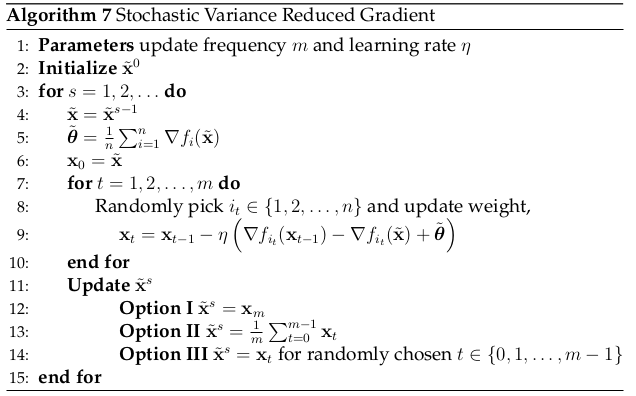
\includegraphics[scale=0.20]{ODS/images/SVRG.png}
\end{wrapfigure}
\textbf{SAGA}:The idea of SAGA is similar to SAG except that SAGA uses a different coefficient to keep the gradient estimator unbiased. SAGA works as follows: $\xx_{t+1} = \xx_t - \gamma\Big[(\nabla f_{i_t}(\xx_t) - \vv_{i_t}^{t-1})$ $  +\frac{1}{n}\sum_{i=1}^n{\vv_i^{t-1}} \Big]$. \\
\textbf{SVRG}: The idea of the algorithm is to use fixed reference point to build the variance-reduced gradient: $\vecg_t = \nabla f_{i_t}(\xx_t) - \nabla f_{i_t}(\Tilde{\xx}) + \nabla F(\Tilde{x})$, where the reference point $\Tilde{\xx}$ is only updated once a while. \\
\textbf{Convergence}: Assume $f_i(\xx)$ is convex and $L$-smooth and $F(\xx)= \frac{1}{n}\sum_{i=1}^n{f_i(\xx)}$ is $\mu$-strongly convex. Let $\xx^* = \argmin_{\xx}{F(\xx)}$, assume that $m$ is sufficiently large, and $\eta \leq \frac{1}{2L}$, so that $\rho = \frac{1}{\mu \eta (1 - 2L\eta) m} + \frac{2L \eta}{1 - 2L\eta} < 1$, then then we have geometric convergence in expectation for SVRG under Option II and III: $\E[F(\Tilde{\xx}^s) - F(\xx^*)] \leq \rho^s [F(\Tilde{\xx}^0) - F(\xx^*)]$. The trick is to prove the lemma: for any $\xx$ we have: $\frac{1}{n}\sum_{i=1}^n{\norm{\nabla f_i(\xx) - \nabla f_i(\xx^*)}_2^2} \leq 2L(F(\xx) - F(\xx^*))$. $\kappa_{\max} := \frac{L_{\max}}{\mu}$. \\

\section{Min-Max Optimization}
We consider the \textbf{min-max problem} of the form $\min_{\xx \in \X} \max{\yy \in \Y} \phi(\xx, \yy)$.
\begin{framed}
    We say that $(\xx^*, \yy^*)$ is a \textbf{saddle point} if $\phi(\xx^*, \yy) \leq \phi(\xx^*, \yy^*) \leq \phi(\xx, \yy^*)$, for any $\xx \in \X$ and $\yy \in \Y$. This can be seen as a \textbf{Nash equilibrium} in a similtaneous game, where no player has an incentive to make unilateral change at the NE.
\end{framed}
\begin{framed}
    We say that $(\xx^*, \yy^*)$ is a \textbf{global minimax point} if $\phi(\xx^*, \yy) \leq \phi(\xx^*, \yy^*) \leq \max_{\yy' \in \Y} \phi(\xx, \yy')$ for any $\xx \in \X, \yy \in \Y$. This can be seen as a \textbf{Stackelberg equilibrium} in a sequential game (best reponse to best reponse).
\end{framed}
Next we define the \textbf{primal} and \textbf{dual} problems induced by the minimax optimization problem:
$\mathrm{Opt}(P) = \min_{\xx \in \X}{\Bar{\phi}(\xx)}$, with $\Bar{\phi}(\xx) = \max_{\yy \in \Y}{\phi(\xx, \yy)}$ and $\mathrm{Opt}(D) = \min_{\xx \in \X}{\ubar{\phi}(\xx)}$, with $\ubar{\phi}(\xx) = \max_{\yy \in \Y}{\phi(\xx, \yy)}$ \\
Notice that weak duality holds ($\mathrm{Opt}(D) \leq \mathrm{Opt}(P)$) and hence: $\max_{\yy \in \Y}\min_{\xx \in X}{\phi(\xx, \yy)} \leq \min_{\xx \in X}\max_{\yy \in \Y}{\phi(\xx, \yy)}$. \\
\textbf{Existence of saddle point}: The point $(\xx^*, \yy^*)$ is a saddle point of $\phi(\xx, \yy)$ if and only if $\max_{\yy \in \Y}\min_{\xx \in X}{\phi(\xx, \yy)} = \min_{\xx \in X}\max_{\yy \in \Y}{\phi(\xx, \yy)}$ and $\xx^* \in \argmin_{\xx \in \X}{\Bar{\phi}(\xx)}$ and $\yy^* \in \argmax_{\yy \in \Y}{\ubar{\phi}(\yy)}$. In other words, $(\xx^*, \yy^*)$ is a saddle point if and only if strong duality holds and $\xx^*$ , $\yy^*$ are respectively the optimal solutions to the induced primal problem (P ) and the dual problem (D). \\
\textbf{Remark}: A saddle point, if it exists, is also a global minimax point.And there is no advantage to the players of knowing the opponent’s choice or to play second. The minimax, maximin, and the equilibrium all give the same payoff. \\
\Title{Minimax Theorem}
\begin{framed}
    \textbf{von Neumann’s Minimax theorem}: For any payoff matrix $A \in \R^{m \times n}$: $\min_{\xx \in \Delta_m} \max_{\yy \in \Delta_n} \xx^T A \yy = \max_{\yy \in \Delta_n} \min_{\xx \in \Delta_m} \xx^T A \yy$, where $\Delta_m = \{ \xx \in \R_{+}^m : \sum_{i=1}^m{x_i} = 1\}, \Delta_n = \{ \yy \in \R_{+}^n : \sum_{i=1}^m{y_i} = 1\}$.
\end{framed}
\begin{framed}
    \textbf{Sion-Kakutani Minimax theorem}: Let sets $\X \subseteq \R^m$ and $\Y \subseteq \R^n$ be two convex compact sets. Let $\phi(\xx, \yy) : \mathcal{X} \cross \mathcal{Y} \rightarrow \R$ be a continuous function such that for any fixed $\yy  \in \Y$ it is convex in $\xx$ and for any fixed $\xx \in \X$ it is convex in $\yy$, we call such a function \textbf{convex-concave}. Then $\phi(\xx, \yy)$ has a saddle point on $\X \times \Y$ and $\max_{\yy \in \Y}\min_{\xx \in X}{\phi(\xx, \yy)} = \min_{\xx \in X}\max_{\yy \in \Y}{\phi(\xx, \yy)}$.
\end{framed}
A function $\phi : \X \times \Y \rightarrow \R$ is \textbf{strongly-convex-strongly-concave} if there exist constants $\mu_1, \mu_2 > 0$ such that: $\phi(\xx, \yy)$ is $\mu_1$-strongly convex in $\xx \in \X$ for every fixed $\yy \in \Y$;  $\phi(\xx, \yy)$ is $\mu_2$-strongly concave in $\yy \in \Y$ for every fixed $\xx \in \X$, namely for any $\xx, \xx_1, \xx_2 \in \X$ and $\yy, \yy_1, \yy_2 \in \Y$:
\begin{enumerate}[label=(\roman*), topsep=0pt,itemsep=0ex,partopsep=0ex,parsep=0ex] 
    \itemsep0em
    \item $\phi(\xx_1, \yy) \geq \phi(\xx_2, \yy) + \nabla_{\xx} \phi(\xx_2, \yy)^T(\xx_1 - \xx_2) + \frac{\mu_1}{2}\norm{\xx_1 - \xx_2}^2$
    \item $- \phi(\xx, \yy_1) \geq - \phi(\xx, \yy_2) - \nabla_{\yy} \phi(\xx, \yy_2)^T(\yy_1 - \yy_2) + \frac{\mu_2}{2}\norm{\yy_1 - \yy_2}^2$
\end{enumerate}
A function $\phi : \X \times \Y \rightarrow \R$ is \textbf{$L$-Lipschitz smooth jointly in $\xx$ and $\yy$} if for any $\xx_1, \xx_2 \in \X$ and $\yy_1, \yy_2 \in \Y$:
\begin{enumerate}[label=(\roman*), topsep=0pt,itemsep=0ex,partopsep=0ex,parsep=0ex] 
    \itemsep0em
    \item $\norm{\nabla_{\xx} \phi(\xx_1, \yy_1) - \nabla_{\xx} \phi(\xx_2, \yy_2)} \leq L (\norm{\xx_1 - \xx_2} + \norm{\yy_1 - \yy_2} )$
    \item $\norm{\nabla_{\yy} \phi(\xx_1, \yy_1) - \nabla_{\yy} \phi(\xx_2, \yy_2)} \leq L (\norm{\xx_1 - \xx_2} + \norm{\yy_1 - \yy_2} )$
\end{enumerate}
We measure the optimality via the \textbf{duality gap}: $\text{duality gap} = \max_{\yy \in \Y} \phi(\widehat{\xx}, \yy) - \min_{\xx \in \X} \phi(\xx, \widehat{\yy}) \geq 0$. When duality gap $=0$ we have a saddle-point. If duality gap $\leq \epsilon$ we have an $\epsilon$-saddle point. \\
\Title{Algorithms}
\begin{framed}
    \textbf{Gradient Descent Ascent}: The algorithm updates x and y simultaneuous at each iteration using
only the gradient information: $\xx_{t+1} = \Pi_{\X}(\xx_t - \eta \nabla_{\xx} \phi(\xx_t, \yy_t))$ and $\yy_{t+1} = \Pi_{\Y}(\yy_t - \eta \nabla_{\yy} \phi(\xx_t, \yy_t))$.
\end{framed}
\textbf{Convergence of GDA}: Assume that $\phi$ is $\mu$-strongly-convex-strongly-concave and jointly smooth with parameter $L$, then GDA with stepsize $\eta < \frac{\mu}{2L^2}$ converges linearly: $ \norm{\xx_{t+1} - \xx^*}^2 + \norm{\yy_{t+1} - \yy^*} \leq (1 + 4\eta^2 L^2 - 2\eta \mu)(\norm{\xx_t - \xx^*}^2 + \norm{\yy_t - \yy^*}^2)$. With stepsize $\eta = \frac{\mu}{4L^2}$ this yields: $\norm{\xx_T - \xx^*}^2 + \norm{\yy_T - \yy^*}^2 \leq (1 - \frac{\mu^2}{4L^2})^T (\norm{\xx_0 - \xx^*}^2 + \norm{\yy_0 - \yy^*}^2)$. \\
\textbf{Careful}: GDA with constant stepsize may not converge for general convex-concave function. Consider the function $\phi(x, y) = xy$. \\
\begin{framed}
    \textbf{Extragradient Method (EG)}: The main idea of EG is to use the gradient at the current point to find a mid-point, and then use the gradient at that mid-point to find the next iterate:
    \begin{enumerate}[label=, topsep=0pt,itemsep=0ex,partopsep=0ex,parsep=0ex, leftmargin=0cm] 
        \itemsep0em
        \item $\xx_{t+\frac{1}{2}} = \Pi_{\X}(\xx_t - \eta \nabla_{\xx} \phi(\xx_t, \yy_t)), \yy_{t+1} = \Pi_{\Y}(\yy_t + \eta \nabla_{\yy} \phi(\xx_t, \yy_t))$,
        \item $\xx_{t+1} = \Pi_{\X}\left(\xx_t - \eta \nabla_{\xx} \phi(\xx_{t+\frac{1}{2}}, \yy_{t + \frac{1}{2}})\right)$, $\yy_{t+1} = \Pi_{\Y}\left(\yy_t - \eta \nabla_{\yy} \phi(\xx_{t+\frac{1}{2}}, \yy_{t + \frac{1}{2}})\right)$.
    \end{enumerate}
\end{framed}
\textbf{Convergence of EG}: Assume that $\D_{\X} := \max_{\xx, \xx'}{\norm{\xx - \xx'}} < \infty$ and $\D_{\Y} := \max_{\yy, \yy'}{\norm{\yy - \yy'}} < \infty$. Assume that $\phi$ is convex-concave and jointly $L$-smooth then EG with stepsize $\eta \leq \frac{1}{2L}$ satisfies by denoting $\widehat{\xx}_T = \frac{1}{T}\sum_{t=1}^T{\xx_{t+\frac{1}{2}}}$ and $\widehat{\yy}_T = \frac{1}{T}\sum_{t=1}^T{\yy_{t+\frac{1}{2}}}$, setting $\eta = \frac{1}{2L}$, this implies that the duality gap: $\epsilon_{\text{sad}}(\widehat{\xx}_T, \widehat{\yy}_T) \leq \frac{D_{\X}^2 + D_{\Y}^2)}{2 \eta T} = \frac{L ( D_{\X}^2 + D_{\Y}^2)}{T}$. \\
\textbf{Connections to Proximal Point Algorithm (PPA)}: At each iteration, PPA performs the update: $(\xx_{t+1}, \yy_{t+1}) = \argmin_{\xx \in \mathcal{X}} \argmax_{\yy \in \mathcal{Y}} \{ \phi(\xx, \yy) + \frac{1}{2\eta}\norm{\xx - \xx_t}^2 - \frac{1}{2\eta}\norm{\yy - \yy_t}^2 \}$. \\
\Title{Variational Inequalities}
\begin{framed}
    \textbf{Variational Inequality (VI) Problem}: Let $\mathcal{Z} \subset \R^d$ be a nonempty subset and consider mapping $F : \mathcal{Z} \rightarrow \R^d$. The goal of a $VI$ is to find a (strong) solution $\zz^* \in \mathcal{Z}$ such that $\langle F(\zz^*), \zz - \zz^* \rangle \geq 0$ for all $\zz \in \mathcal{Z}$. This is known as the \textbf{Stampacchia Variational Inequality (SVI)}. A closely relevant problem is the \textbf{Minty Variational Inequality (MVI)}, which aims to find a (weak) solution $\zz^*$ such that $\langle F(\zz), \zz - \zz^* \rangle \geq 0$ for all $\zz \in \mathcal{Z}$.
\end{framed}
An operator $F : \mathcal{Z} \rightarrow \R^d$ is said to be \textbf{monotone} if $\langle F(\uu) - f(\vv), \uu - \vv \rangle \geq 0$, $\forall \uu, \vv \in \mathcal{Z}$, it is said to be \textbf{$\mu$-strongly monotone} with modulus $\mu > 0$ if $\langle F(\uu) - f(\vv), \uu - \vv \rangle \geq \mu \norm{\uu - \vv}^2$, $\forall \uu, \vv \in \mathcal{Z}$.
\textbf{Equivalence of SVI and MVI} \textit{(i)} If $F$ is monotone, then a solution to SVI is also a solution to MVI. \textit{(ii)} If $F$ is continuous and $\mathcal{Z}$ is convex, then a solution to MVI is also a solution to SVI. \\
\textbf{Accuracy Measure}: A natural inaccuracy measure if a candidate solution $\widehat{\zz}$ to MVI is the dual gap function: $\epsilon_{\text{VI}}(\widehat{\zz}) := \max_{\zz \in \mathcal{Z}} \langle F(\zz), \widehat{\zz} - \zz \rangle$. \\
Extragradient Method (EG) and Optimistic Gradient Descent Ascent (OGDA) can be directly extended to solving VIs. 

%TO-DO: formel für normalverteilung, map estimet, 


% ____ FOOTER __________________________________________________________________
% Template:
%Julia Bogdan (jbogdan@student.ethz.ch), 2022
%
% Content: 
% based on Lecture Introduction to Machine Learning in FS22 @ETH Zürich 

\end{multicols*}
\end{document}
